\documentclass[11pt,a4paper]{article}
\usepackage[a4paper,margin=2cm]{geometry}
\usepackage{amsmath,amssymb}
\usepackage{xcolor}
\usepackage{mdframed}
\usepackage{enumitem}
\usepackage{tikz}
\usepackage{pdflscape}
\usepackage[hidelinks]{hyperref}
\usepackage{titlesec}
\usepackage{fancyhdr}
\renewcommand{\contentsname}{Inhoud}

\definecolor{deepblue}{RGB}{20,40,90}
\definecolor{goldacc}{RGB}{170,130,40}
\definecolor{boxbg}{RGB}{245,247,251}
\definecolor{sealbg}{RGB}{250,240,225}

\titleformat{\section}{\Large\bfseries\color{deepblue}}{\thesection}{0.6em}{}
\titleformat{\subsection}{\large\bfseries\color{deepblue}}{\thesubsection}{0.6em}{}

\pagestyle{fancy}
\fancyhf{}
\renewcommand{\headrulewidth}{0.3pt}
\fancyhead[L]{\small\color{gray}De verborgen matrix}
\fancyhead[R]{\small\color{gray}\thepage}

\newmdenv[backgroundcolor=boxbg, linecolor=deepblue, linewidth=0.8pt, roundcorner=4pt, innermargin=10pt, outermargin=0pt, skipabove=8pt, skipbelow=8pt]{infobox}
\newmdenv[backgroundcolor=sealbg, linecolor=goldacc, linewidth=1pt, roundcorner=4pt, innermargin=12pt, outermargin=0pt, skipabove=8pt, skipbelow=8pt]{sealbox}

\title{\vspace{-2cm}\color{deepblue}\Huge\textbf{De Verborgen Matrix}\\[0.3cm]
\Large\color{goldacc} Een puzzel in lineaire algebra over $\mathrm{GF}(2)$}
\author{}
\date{}

\begin{document}
\maketitle
\thispagestyle{empty}

\vspace{0.3cm}
\begin{center}
\begin{minipage}{0.85\textwidth}
\centering
\textit{Achter twee matrices van 29 bij 29 nullen en enen\\
schuilt een derde matrix, verscholen achter vier fasen van berekening.\\
De enige weg erheen: Gauss-eliminatie, volledig modulo 2.}
\end{minipage}
\end{center}
\vspace{0.8cm}

\tableofcontents
\thispagestyle{empty}
\newpage

\section{De opdracht — overzicht}

Deze keer krijg je matrix $A$ niet cadeau. Je moet ze zelf opbouwen. Het traject verloopt in vier fasen:

\begin{enumerate}
\item \textbf{Los een vergelijking op} om een geheim \emph{sleutelgetal} $S$ te vinden (een getal tussen 0 en $2^{29}-1$).
\item \textbf{Voer $S$ in een schuifregister} (een LFSR — meer hierover in \S3) en genereer daarmee, bit voor bit, twee matrices: matrix $A$ zelf, én een \emph{maskeermatrix} $M$.
\item Je krijgt een \textbf{vercijferde matrix} $B_{\text{enc}}$. Met je zelfgemaakte $M$ demaskeer je die tot de echte matrix $B$.
\item Los tot slot het stelsel $A\cdot X \equiv B \pmod 2$ op via Gauss-eliminatie. De oplossing $X$ is een unieke $29\times 29$-matrix van 0'en en 1'en.
\end{enumerate}

\newpage
\section{Fase 1 — Het sleutelgetal}

Bereken:
\[
S = \frac{2000}{\pi}\sum_{n=0}^{\infty} \frac{(-1)^n}{2n+1}.
\]

\begin{infobox}
\textbf{Wat je nodig hebt voor de volgende fase.} $S$ moet een geheel getal zijn tussen $0$ en $2^{29}-1 = 536\,870\,911$. Zodra je $S$ hebt, zet je het om naar een rij van precies 29 bits (met voorloopnullen indien nodig) — dat wordt de seed voor Fase 2.
\end{infobox}

\newpage
\section{Fase 2 — Van sleutelgetal naar matrices: het LFSR}

\subsection{Wat is een LFSR?}
Een \textbf{lineair-terugkoppelingsschuifregister} (Engels: \emph{linear feedback shift register}, LFSR) is een eenvoudig mechanisme dat een oneindige reeks bits genereert uit een eindig geheugen. Het bestaat uit een rij van $d$ geheugenposities (hier $d=29$), gevuld met een startwaarde (de \emph{seed}). Bij elke stap:
\begin{enumerate}
\item Bereken een \textbf{terugkoppelbit}: de \textsc{xor} van de bits op vaste, vooraf afgesproken posities (de \emph{tap-posities}).
\item Schuif alle bits één positie op.
\item De nieuwe terugkoppelbit komt binnen aan het ene uiteinde; de bit die aan het andere uiteinde ``uitvalt'' is de \textbf{output-bit} van deze stap.
\end{enumerate}
Dit is exact dezelfde soort wiskunde (lineaire recursies modulo 2) als bij stroomvercijfering en foutcorrectie in de cryptografie en codeertheorie — het past dus naadloos bij de rest van deze puzzel.

\textbf{Voor deze puzzel:} register van lengte $d=29$, tap-posities $29$ en $2$ (dit hoort bij de \emph{primitieve veelterm} $x^{29}+x^2+1$ over $\mathrm{GF}(2)$ — een standaardkeuze uit de codeertheorie die garandeert dat de reeks pas na $2^{29}-1$ stappen zichzelf herhaalt).

\subsection{Volledig uitgewerkt minivoorbeeld (register van lengte 4)}
Ter illustratie: een LFSR met $d=4$, tap-posities $4$ en $1$, en seed $1001_2 = 9$. Het register wordt weergegeven als $(r_1,r_2,r_3,r_4)$, met $r_1$ het meest linkse bit.

\begin{center}
\begin{tabular}{c|c|c}
stap & register vóór de stap & output-bit (= $r_4$ vóór schuiven) \\\hline
1 & $(1,0,0,1)$ & $1$ \\
2 & $(0,1,0,0)$ & $0$ \\
3 & $(0,0,1,0)$ & $0$ \\
4 & $(0,0,0,1)$ & $1$ \\
5 & $(1,0,0,0)$ & $0$ \\
6 & $(1,1,0,0)$ & $0$ \\
7 & $(1,1,1,0)$ & $0$ \\
8 & $(1,1,1,1)$ & $1$ \\
\end{tabular}
\end{center}

\textbf{Toelichting bij stap 1:} terugkoppelbit $= r_4 \oplus r_1 = 1 \oplus 1 = 0$. De output-bit van deze stap is het bit dat rechts uitvalt: $r_4 = 1$. Na het schuiven wordt het nieuwe register $(0,\,1,\,0,\,0)$ — de terugkoppelbit ($0$) komt links binnen, en $r_1,r_2,r_3$ schuiven één plaats op.

\textbf{Toelichting bij stap 4:} register is $(0,0,0,1)$. Terugkoppelbit $=r_4\oplus r_1 = 1\oplus 0=1$. Output-bit $=r_4=1$. Nieuw register: $(1,0,0,0)$.

De resulterende bitreeks na 8 stappen: $1,0,0,1,0,0,0,1,\dots$ Dit proces zet je nu voort voor de echte puzzel — maar met een register van lengte 29, tap-posities 29 en 2, en de seed uit Fase 1.

\subsection{Van bitreeks naar matrices}
Start het register met de 29-bits seed die je in Fase 1 hebt gevonden (het meest linkse bit is $r_1$). Genereer op de hierboven beschreven manier een reeks van minstens $1682$ output-bits.

\begin{itemize}
\item De \textbf{eerste 841 bits} vul je, rij voor rij, in een rooster van $29\times 29$ — dit wordt matrix $A$.
\item De \textbf{volgende 841 bits} (bit 842 t.e.m. 1682) vul je op dezelfde manier in een tweede rooster van $29\times 29$ — dit wordt de maskeermatrix $M$.
\end{itemize}

\begin{infobox}
\textbf{Zelfcontrole.} Tel, ter controle, het totaal aantal enen in je matrices:
\begin{itemize}
\item Matrix $A$ moet exact \textbf{421} enen bevatten (op 841 cellen).
\item Matrix $M$ moet exact \textbf{416} enen bevatten (op 841 cellen).
\end{itemize}
Klopt dit niet? Zoek dan eerst de fout in je bitreeks voor je verdergaat — een enkele omgewisselde bit vroeg in de reeks verschuift alles wat erna komt.
\end{infobox}

\newpage
\subsection{Invulrooster — matrix \texorpdfstring{$A$}{A}}
Vul hier, rij voor rij, de eerste 841 output-bits in (bit 1 bovenaan-links, verder rij per rij).

\begin{center}
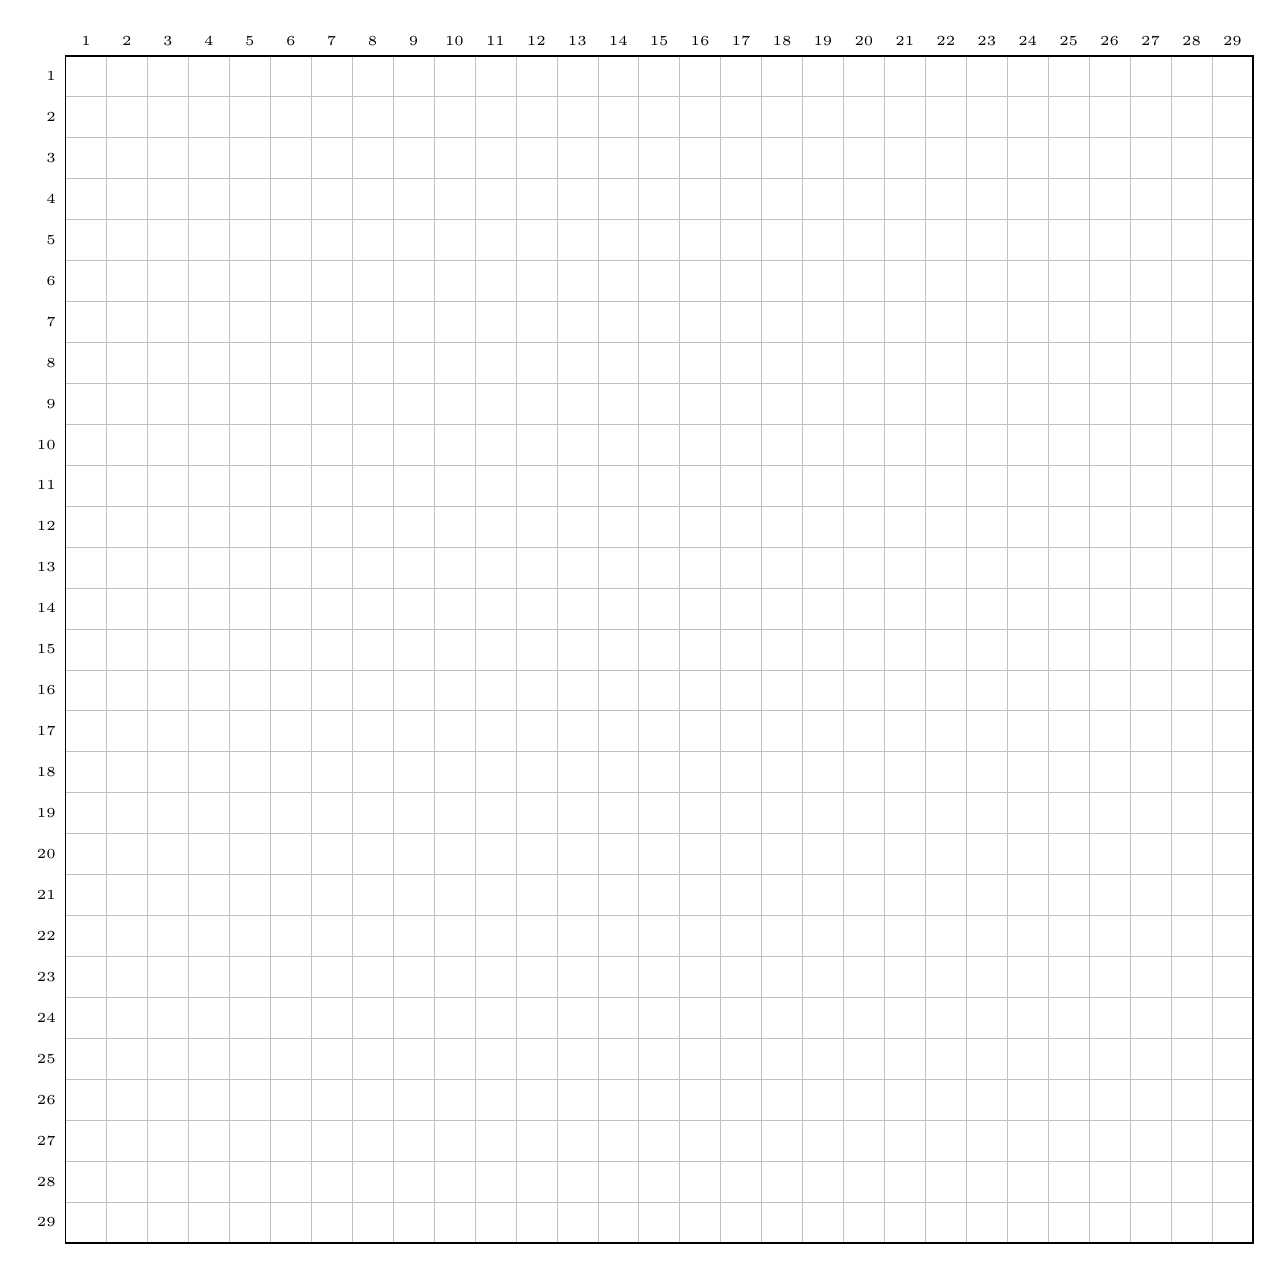
\begin{tikzpicture}[x=0.52cm,y=-0.52cm,font=\tiny]
\draw[gray!50,line width=0.2pt] (0,0) -- (0,29);
\draw[gray!50,line width=0.2pt] (1,0) -- (1,29);
\draw[gray!50,line width=0.2pt] (2,0) -- (2,29);
\draw[gray!50,line width=0.2pt] (3,0) -- (3,29);
\draw[gray!50,line width=0.2pt] (4,0) -- (4,29);
\draw[gray!50,line width=0.2pt] (5,0) -- (5,29);
\draw[gray!50,line width=0.2pt] (6,0) -- (6,29);
\draw[gray!50,line width=0.2pt] (7,0) -- (7,29);
\draw[gray!50,line width=0.2pt] (8,0) -- (8,29);
\draw[gray!50,line width=0.2pt] (9,0) -- (9,29);
\draw[gray!50,line width=0.2pt] (10,0) -- (10,29);
\draw[gray!50,line width=0.2pt] (11,0) -- (11,29);
\draw[gray!50,line width=0.2pt] (12,0) -- (12,29);
\draw[gray!50,line width=0.2pt] (13,0) -- (13,29);
\draw[gray!50,line width=0.2pt] (14,0) -- (14,29);
\draw[gray!50,line width=0.2pt] (15,0) -- (15,29);
\draw[gray!50,line width=0.2pt] (16,0) -- (16,29);
\draw[gray!50,line width=0.2pt] (17,0) -- (17,29);
\draw[gray!50,line width=0.2pt] (18,0) -- (18,29);
\draw[gray!50,line width=0.2pt] (19,0) -- (19,29);
\draw[gray!50,line width=0.2pt] (20,0) -- (20,29);
\draw[gray!50,line width=0.2pt] (21,0) -- (21,29);
\draw[gray!50,line width=0.2pt] (22,0) -- (22,29);
\draw[gray!50,line width=0.2pt] (23,0) -- (23,29);
\draw[gray!50,line width=0.2pt] (24,0) -- (24,29);
\draw[gray!50,line width=0.2pt] (25,0) -- (25,29);
\draw[gray!50,line width=0.2pt] (26,0) -- (26,29);
\draw[gray!50,line width=0.2pt] (27,0) -- (27,29);
\draw[gray!50,line width=0.2pt] (28,0) -- (28,29);
\draw[gray!50,line width=0.2pt] (29,0) -- (29,29);
\draw[gray!50,line width=0.2pt] (0,0) -- (29,0);
\draw[gray!50,line width=0.2pt] (0,1) -- (29,1);
\draw[gray!50,line width=0.2pt] (0,2) -- (29,2);
\draw[gray!50,line width=0.2pt] (0,3) -- (29,3);
\draw[gray!50,line width=0.2pt] (0,4) -- (29,4);
\draw[gray!50,line width=0.2pt] (0,5) -- (29,5);
\draw[gray!50,line width=0.2pt] (0,6) -- (29,6);
\draw[gray!50,line width=0.2pt] (0,7) -- (29,7);
\draw[gray!50,line width=0.2pt] (0,8) -- (29,8);
\draw[gray!50,line width=0.2pt] (0,9) -- (29,9);
\draw[gray!50,line width=0.2pt] (0,10) -- (29,10);
\draw[gray!50,line width=0.2pt] (0,11) -- (29,11);
\draw[gray!50,line width=0.2pt] (0,12) -- (29,12);
\draw[gray!50,line width=0.2pt] (0,13) -- (29,13);
\draw[gray!50,line width=0.2pt] (0,14) -- (29,14);
\draw[gray!50,line width=0.2pt] (0,15) -- (29,15);
\draw[gray!50,line width=0.2pt] (0,16) -- (29,16);
\draw[gray!50,line width=0.2pt] (0,17) -- (29,17);
\draw[gray!50,line width=0.2pt] (0,18) -- (29,18);
\draw[gray!50,line width=0.2pt] (0,19) -- (29,19);
\draw[gray!50,line width=0.2pt] (0,20) -- (29,20);
\draw[gray!50,line width=0.2pt] (0,21) -- (29,21);
\draw[gray!50,line width=0.2pt] (0,22) -- (29,22);
\draw[gray!50,line width=0.2pt] (0,23) -- (29,23);
\draw[gray!50,line width=0.2pt] (0,24) -- (29,24);
\draw[gray!50,line width=0.2pt] (0,25) -- (29,25);
\draw[gray!50,line width=0.2pt] (0,26) -- (29,26);
\draw[gray!50,line width=0.2pt] (0,27) -- (29,27);
\draw[gray!50,line width=0.2pt] (0,28) -- (29,28);
\draw[gray!50,line width=0.2pt] (0,29) -- (29,29);
\draw[black,line width=0.7pt] (0,0) rectangle (29,29);
\node[above] at (0.5,0) {\tiny 1};
\node[above] at (1.5,0) {\tiny 2};
\node[above] at (2.5,0) {\tiny 3};
\node[above] at (3.5,0) {\tiny 4};
\node[above] at (4.5,0) {\tiny 5};
\node[above] at (5.5,0) {\tiny 6};
\node[above] at (6.5,0) {\tiny 7};
\node[above] at (7.5,0) {\tiny 8};
\node[above] at (8.5,0) {\tiny 9};
\node[above] at (9.5,0) {\tiny 10};
\node[above] at (10.5,0) {\tiny 11};
\node[above] at (11.5,0) {\tiny 12};
\node[above] at (12.5,0) {\tiny 13};
\node[above] at (13.5,0) {\tiny 14};
\node[above] at (14.5,0) {\tiny 15};
\node[above] at (15.5,0) {\tiny 16};
\node[above] at (16.5,0) {\tiny 17};
\node[above] at (17.5,0) {\tiny 18};
\node[above] at (18.5,0) {\tiny 19};
\node[above] at (19.5,0) {\tiny 20};
\node[above] at (20.5,0) {\tiny 21};
\node[above] at (21.5,0) {\tiny 22};
\node[above] at (22.5,0) {\tiny 23};
\node[above] at (23.5,0) {\tiny 24};
\node[above] at (24.5,0) {\tiny 25};
\node[above] at (25.5,0) {\tiny 26};
\node[above] at (26.5,0) {\tiny 27};
\node[above] at (27.5,0) {\tiny 28};
\node[above] at (28.5,0) {\tiny 29};
\node[left] at (0,0.5) {\tiny 1};
\node[left] at (0,1.5) {\tiny 2};
\node[left] at (0,2.5) {\tiny 3};
\node[left] at (0,3.5) {\tiny 4};
\node[left] at (0,4.5) {\tiny 5};
\node[left] at (0,5.5) {\tiny 6};
\node[left] at (0,6.5) {\tiny 7};
\node[left] at (0,7.5) {\tiny 8};
\node[left] at (0,8.5) {\tiny 9};
\node[left] at (0,9.5) {\tiny 10};
\node[left] at (0,10.5) {\tiny 11};
\node[left] at (0,11.5) {\tiny 12};
\node[left] at (0,12.5) {\tiny 13};
\node[left] at (0,13.5) {\tiny 14};
\node[left] at (0,14.5) {\tiny 15};
\node[left] at (0,15.5) {\tiny 16};
\node[left] at (0,16.5) {\tiny 17};
\node[left] at (0,17.5) {\tiny 18};
\node[left] at (0,18.5) {\tiny 19};
\node[left] at (0,19.5) {\tiny 20};
\node[left] at (0,20.5) {\tiny 21};
\node[left] at (0,21.5) {\tiny 22};
\node[left] at (0,22.5) {\tiny 23};
\node[left] at (0,23.5) {\tiny 24};
\node[left] at (0,24.5) {\tiny 25};
\node[left] at (0,25.5) {\tiny 26};
\node[left] at (0,26.5) {\tiny 27};
\node[left] at (0,27.5) {\tiny 28};
\node[left] at (0,28.5) {\tiny 29};
\end{tikzpicture}
\end{center}

\newpage
\subsection{Invulrooster — maskeermatrix \texorpdfstring{$M$}{M}}
Vul hier, rij voor rij, bit 842 t.e.m.\ 1682 in.

\begin{center}
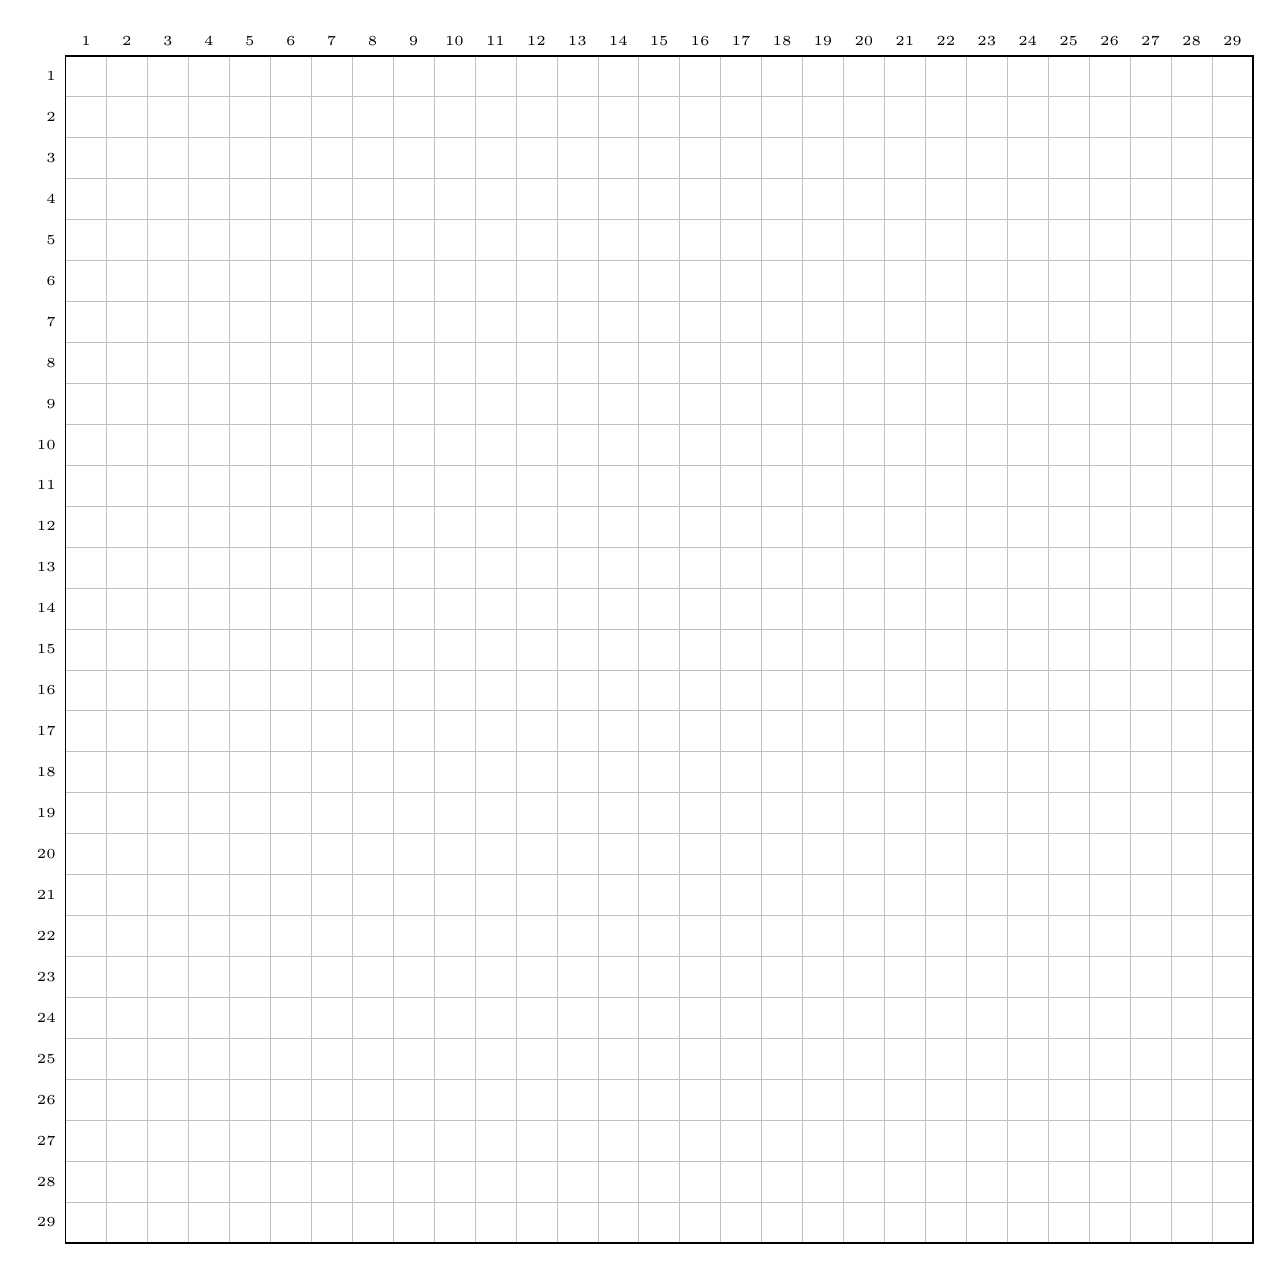
\begin{tikzpicture}[x=0.52cm,y=-0.52cm,font=\tiny]
\draw[gray!50,line width=0.2pt] (0,0) -- (0,29);
\draw[gray!50,line width=0.2pt] (1,0) -- (1,29);
\draw[gray!50,line width=0.2pt] (2,0) -- (2,29);
\draw[gray!50,line width=0.2pt] (3,0) -- (3,29);
\draw[gray!50,line width=0.2pt] (4,0) -- (4,29);
\draw[gray!50,line width=0.2pt] (5,0) -- (5,29);
\draw[gray!50,line width=0.2pt] (6,0) -- (6,29);
\draw[gray!50,line width=0.2pt] (7,0) -- (7,29);
\draw[gray!50,line width=0.2pt] (8,0) -- (8,29);
\draw[gray!50,line width=0.2pt] (9,0) -- (9,29);
\draw[gray!50,line width=0.2pt] (10,0) -- (10,29);
\draw[gray!50,line width=0.2pt] (11,0) -- (11,29);
\draw[gray!50,line width=0.2pt] (12,0) -- (12,29);
\draw[gray!50,line width=0.2pt] (13,0) -- (13,29);
\draw[gray!50,line width=0.2pt] (14,0) -- (14,29);
\draw[gray!50,line width=0.2pt] (15,0) -- (15,29);
\draw[gray!50,line width=0.2pt] (16,0) -- (16,29);
\draw[gray!50,line width=0.2pt] (17,0) -- (17,29);
\draw[gray!50,line width=0.2pt] (18,0) -- (18,29);
\draw[gray!50,line width=0.2pt] (19,0) -- (19,29);
\draw[gray!50,line width=0.2pt] (20,0) -- (20,29);
\draw[gray!50,line width=0.2pt] (21,0) -- (21,29);
\draw[gray!50,line width=0.2pt] (22,0) -- (22,29);
\draw[gray!50,line width=0.2pt] (23,0) -- (23,29);
\draw[gray!50,line width=0.2pt] (24,0) -- (24,29);
\draw[gray!50,line width=0.2pt] (25,0) -- (25,29);
\draw[gray!50,line width=0.2pt] (26,0) -- (26,29);
\draw[gray!50,line width=0.2pt] (27,0) -- (27,29);
\draw[gray!50,line width=0.2pt] (28,0) -- (28,29);
\draw[gray!50,line width=0.2pt] (29,0) -- (29,29);
\draw[gray!50,line width=0.2pt] (0,0) -- (29,0);
\draw[gray!50,line width=0.2pt] (0,1) -- (29,1);
\draw[gray!50,line width=0.2pt] (0,2) -- (29,2);
\draw[gray!50,line width=0.2pt] (0,3) -- (29,3);
\draw[gray!50,line width=0.2pt] (0,4) -- (29,4);
\draw[gray!50,line width=0.2pt] (0,5) -- (29,5);
\draw[gray!50,line width=0.2pt] (0,6) -- (29,6);
\draw[gray!50,line width=0.2pt] (0,7) -- (29,7);
\draw[gray!50,line width=0.2pt] (0,8) -- (29,8);
\draw[gray!50,line width=0.2pt] (0,9) -- (29,9);
\draw[gray!50,line width=0.2pt] (0,10) -- (29,10);
\draw[gray!50,line width=0.2pt] (0,11) -- (29,11);
\draw[gray!50,line width=0.2pt] (0,12) -- (29,12);
\draw[gray!50,line width=0.2pt] (0,13) -- (29,13);
\draw[gray!50,line width=0.2pt] (0,14) -- (29,14);
\draw[gray!50,line width=0.2pt] (0,15) -- (29,15);
\draw[gray!50,line width=0.2pt] (0,16) -- (29,16);
\draw[gray!50,line width=0.2pt] (0,17) -- (29,17);
\draw[gray!50,line width=0.2pt] (0,18) -- (29,18);
\draw[gray!50,line width=0.2pt] (0,19) -- (29,19);
\draw[gray!50,line width=0.2pt] (0,20) -- (29,20);
\draw[gray!50,line width=0.2pt] (0,21) -- (29,21);
\draw[gray!50,line width=0.2pt] (0,22) -- (29,22);
\draw[gray!50,line width=0.2pt] (0,23) -- (29,23);
\draw[gray!50,line width=0.2pt] (0,24) -- (29,24);
\draw[gray!50,line width=0.2pt] (0,25) -- (29,25);
\draw[gray!50,line width=0.2pt] (0,26) -- (29,26);
\draw[gray!50,line width=0.2pt] (0,27) -- (29,27);
\draw[gray!50,line width=0.2pt] (0,28) -- (29,28);
\draw[gray!50,line width=0.2pt] (0,29) -- (29,29);
\draw[black,line width=0.7pt] (0,0) rectangle (29,29);
\node[above] at (0.5,0) {\tiny 1};
\node[above] at (1.5,0) {\tiny 2};
\node[above] at (2.5,0) {\tiny 3};
\node[above] at (3.5,0) {\tiny 4};
\node[above] at (4.5,0) {\tiny 5};
\node[above] at (5.5,0) {\tiny 6};
\node[above] at (6.5,0) {\tiny 7};
\node[above] at (7.5,0) {\tiny 8};
\node[above] at (8.5,0) {\tiny 9};
\node[above] at (9.5,0) {\tiny 10};
\node[above] at (10.5,0) {\tiny 11};
\node[above] at (11.5,0) {\tiny 12};
\node[above] at (12.5,0) {\tiny 13};
\node[above] at (13.5,0) {\tiny 14};
\node[above] at (14.5,0) {\tiny 15};
\node[above] at (15.5,0) {\tiny 16};
\node[above] at (16.5,0) {\tiny 17};
\node[above] at (17.5,0) {\tiny 18};
\node[above] at (18.5,0) {\tiny 19};
\node[above] at (19.5,0) {\tiny 20};
\node[above] at (20.5,0) {\tiny 21};
\node[above] at (21.5,0) {\tiny 22};
\node[above] at (22.5,0) {\tiny 23};
\node[above] at (23.5,0) {\tiny 24};
\node[above] at (24.5,0) {\tiny 25};
\node[above] at (25.5,0) {\tiny 26};
\node[above] at (26.5,0) {\tiny 27};
\node[above] at (27.5,0) {\tiny 28};
\node[above] at (28.5,0) {\tiny 29};
\node[left] at (0,0.5) {\tiny 1};
\node[left] at (0,1.5) {\tiny 2};
\node[left] at (0,2.5) {\tiny 3};
\node[left] at (0,3.5) {\tiny 4};
\node[left] at (0,4.5) {\tiny 5};
\node[left] at (0,5.5) {\tiny 6};
\node[left] at (0,6.5) {\tiny 7};
\node[left] at (0,7.5) {\tiny 8};
\node[left] at (0,8.5) {\tiny 9};
\node[left] at (0,9.5) {\tiny 10};
\node[left] at (0,10.5) {\tiny 11};
\node[left] at (0,11.5) {\tiny 12};
\node[left] at (0,12.5) {\tiny 13};
\node[left] at (0,13.5) {\tiny 14};
\node[left] at (0,14.5) {\tiny 15};
\node[left] at (0,15.5) {\tiny 16};
\node[left] at (0,16.5) {\tiny 17};
\node[left] at (0,17.5) {\tiny 18};
\node[left] at (0,18.5) {\tiny 19};
\node[left] at (0,19.5) {\tiny 20};
\node[left] at (0,20.5) {\tiny 21};
\node[left] at (0,21.5) {\tiny 22};
\node[left] at (0,22.5) {\tiny 23};
\node[left] at (0,23.5) {\tiny 24};
\node[left] at (0,24.5) {\tiny 25};
\node[left] at (0,25.5) {\tiny 26};
\node[left] at (0,26.5) {\tiny 27};
\node[left] at (0,27.5) {\tiny 28};
\node[left] at (0,28.5) {\tiny 29};
\end{tikzpicture}
\end{center}

\newpage
\section{Fase 3 — De vercijferde matrix demaskeren}

Je krijgt hieronder niet matrix $B$ zelf, maar een \textbf{vercijferde versie} $B_{\text{enc}}$. Deze is ontstaan door de echte matrix $B$ bit voor bit te \textsc{xor}-en met jouw maskeermatrix $M$:
\[
B_{\text{enc}} = B \oplus M \pmod 2.
\]
Omdat \textsc{xor} zijn eigen inverse is ($a\oplus b\oplus b = a$), geldt: zodra je $M$ hebt (uit Fase 2), demaskeer je met exact dezelfde operatie:
\[
B = B_{\text{enc}} \oplus M \pmod 2.
\]
Bereken dit cel voor cel (841 keer \textsc{xor}) om de echte matrix $B$ te bekomen.

\begin{infobox}
De echte matrix $B$ moet, ter controle, exact \textbf{459} enen bevatten.
\end{infobox}

\subsection*{De vercijferde matrix \texorpdfstring{$B_{\text{enc}}$}{B enc}}
\begin{center}
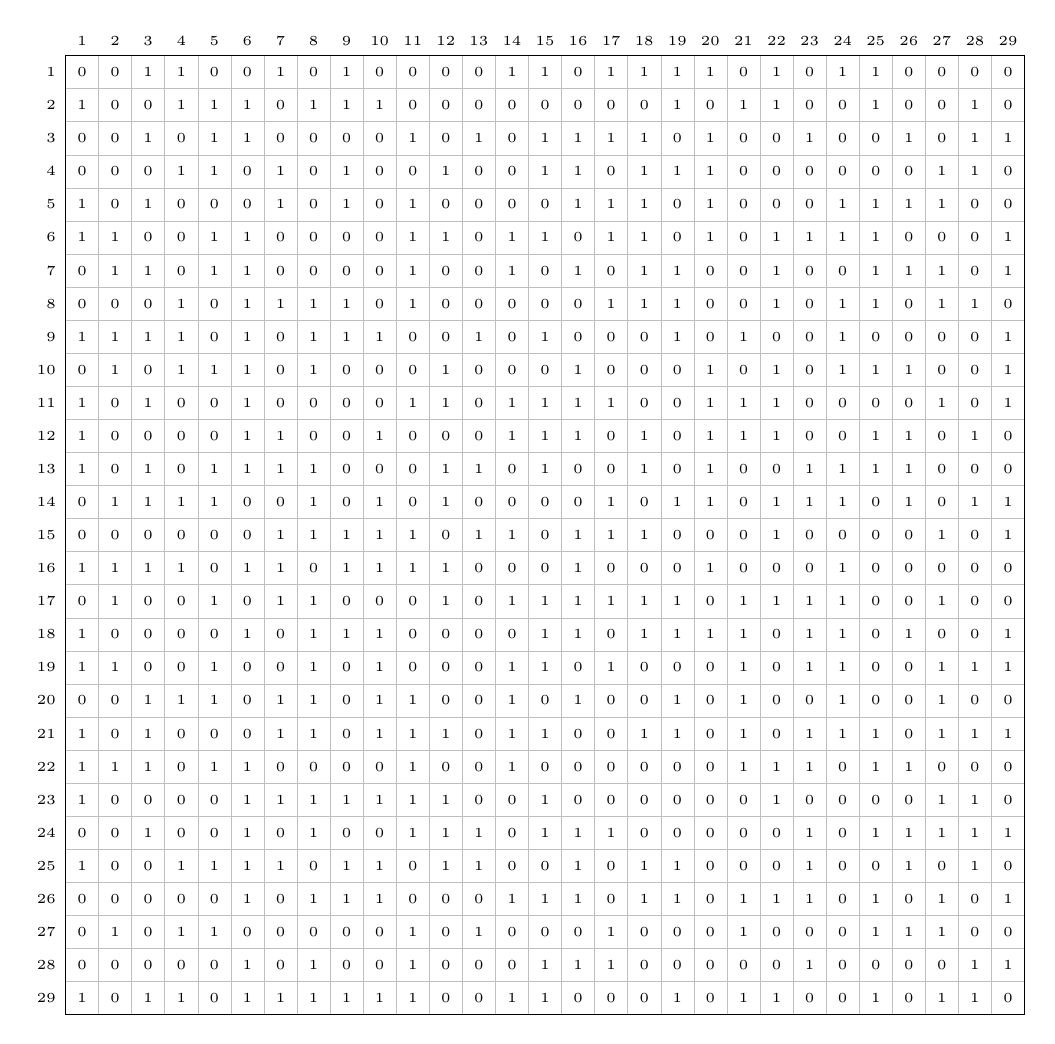
\begin{tikzpicture}[x=0.42cm,y=-0.42cm,font=\tiny]
\draw[gray!50,line width=0.2pt] (0,0) -- (0,29);
\draw[gray!50,line width=0.2pt] (1,0) -- (1,29);
\draw[gray!50,line width=0.2pt] (2,0) -- (2,29);
\draw[gray!50,line width=0.2pt] (3,0) -- (3,29);
\draw[gray!50,line width=0.2pt] (4,0) -- (4,29);
\draw[gray!50,line width=0.2pt] (5,0) -- (5,29);
\draw[gray!50,line width=0.2pt] (6,0) -- (6,29);
\draw[gray!50,line width=0.2pt] (7,0) -- (7,29);
\draw[gray!50,line width=0.2pt] (8,0) -- (8,29);
\draw[gray!50,line width=0.2pt] (9,0) -- (9,29);
\draw[gray!50,line width=0.2pt] (10,0) -- (10,29);
\draw[gray!50,line width=0.2pt] (11,0) -- (11,29);
\draw[gray!50,line width=0.2pt] (12,0) -- (12,29);
\draw[gray!50,line width=0.2pt] (13,0) -- (13,29);
\draw[gray!50,line width=0.2pt] (14,0) -- (14,29);
\draw[gray!50,line width=0.2pt] (15,0) -- (15,29);
\draw[gray!50,line width=0.2pt] (16,0) -- (16,29);
\draw[gray!50,line width=0.2pt] (17,0) -- (17,29);
\draw[gray!50,line width=0.2pt] (18,0) -- (18,29);
\draw[gray!50,line width=0.2pt] (19,0) -- (19,29);
\draw[gray!50,line width=0.2pt] (20,0) -- (20,29);
\draw[gray!50,line width=0.2pt] (21,0) -- (21,29);
\draw[gray!50,line width=0.2pt] (22,0) -- (22,29);
\draw[gray!50,line width=0.2pt] (23,0) -- (23,29);
\draw[gray!50,line width=0.2pt] (24,0) -- (24,29);
\draw[gray!50,line width=0.2pt] (25,0) -- (25,29);
\draw[gray!50,line width=0.2pt] (26,0) -- (26,29);
\draw[gray!50,line width=0.2pt] (27,0) -- (27,29);
\draw[gray!50,line width=0.2pt] (28,0) -- (28,29);
\draw[gray!50,line width=0.2pt] (29,0) -- (29,29);
\draw[gray!50,line width=0.2pt] (0,0) -- (29,0);
\draw[gray!50,line width=0.2pt] (0,1) -- (29,1);
\draw[gray!50,line width=0.2pt] (0,2) -- (29,2);
\draw[gray!50,line width=0.2pt] (0,3) -- (29,3);
\draw[gray!50,line width=0.2pt] (0,4) -- (29,4);
\draw[gray!50,line width=0.2pt] (0,5) -- (29,5);
\draw[gray!50,line width=0.2pt] (0,6) -- (29,6);
\draw[gray!50,line width=0.2pt] (0,7) -- (29,7);
\draw[gray!50,line width=0.2pt] (0,8) -- (29,8);
\draw[gray!50,line width=0.2pt] (0,9) -- (29,9);
\draw[gray!50,line width=0.2pt] (0,10) -- (29,10);
\draw[gray!50,line width=0.2pt] (0,11) -- (29,11);
\draw[gray!50,line width=0.2pt] (0,12) -- (29,12);
\draw[gray!50,line width=0.2pt] (0,13) -- (29,13);
\draw[gray!50,line width=0.2pt] (0,14) -- (29,14);
\draw[gray!50,line width=0.2pt] (0,15) -- (29,15);
\draw[gray!50,line width=0.2pt] (0,16) -- (29,16);
\draw[gray!50,line width=0.2pt] (0,17) -- (29,17);
\draw[gray!50,line width=0.2pt] (0,18) -- (29,18);
\draw[gray!50,line width=0.2pt] (0,19) -- (29,19);
\draw[gray!50,line width=0.2pt] (0,20) -- (29,20);
\draw[gray!50,line width=0.2pt] (0,21) -- (29,21);
\draw[gray!50,line width=0.2pt] (0,22) -- (29,22);
\draw[gray!50,line width=0.2pt] (0,23) -- (29,23);
\draw[gray!50,line width=0.2pt] (0,24) -- (29,24);
\draw[gray!50,line width=0.2pt] (0,25) -- (29,25);
\draw[gray!50,line width=0.2pt] (0,26) -- (29,26);
\draw[gray!50,line width=0.2pt] (0,27) -- (29,27);
\draw[gray!50,line width=0.2pt] (0,28) -- (29,28);
\draw[gray!50,line width=0.2pt] (0,29) -- (29,29);
\draw[black,line width=0.6pt] (0,0) rectangle (29,29);
\node[above] at (0.5,0) {\tiny 1};
\node[above] at (1.5,0) {\tiny 2};
\node[above] at (2.5,0) {\tiny 3};
\node[above] at (3.5,0) {\tiny 4};
\node[above] at (4.5,0) {\tiny 5};
\node[above] at (5.5,0) {\tiny 6};
\node[above] at (6.5,0) {\tiny 7};
\node[above] at (7.5,0) {\tiny 8};
\node[above] at (8.5,0) {\tiny 9};
\node[above] at (9.5,0) {\tiny 10};
\node[above] at (10.5,0) {\tiny 11};
\node[above] at (11.5,0) {\tiny 12};
\node[above] at (12.5,0) {\tiny 13};
\node[above] at (13.5,0) {\tiny 14};
\node[above] at (14.5,0) {\tiny 15};
\node[above] at (15.5,0) {\tiny 16};
\node[above] at (16.5,0) {\tiny 17};
\node[above] at (17.5,0) {\tiny 18};
\node[above] at (18.5,0) {\tiny 19};
\node[above] at (19.5,0) {\tiny 20};
\node[above] at (20.5,0) {\tiny 21};
\node[above] at (21.5,0) {\tiny 22};
\node[above] at (22.5,0) {\tiny 23};
\node[above] at (23.5,0) {\tiny 24};
\node[above] at (24.5,0) {\tiny 25};
\node[above] at (25.5,0) {\tiny 26};
\node[above] at (26.5,0) {\tiny 27};
\node[above] at (27.5,0) {\tiny 28};
\node[above] at (28.5,0) {\tiny 29};
\node[left] at (0,0.5) {\tiny 1};
\node[left] at (0,1.5) {\tiny 2};
\node[left] at (0,2.5) {\tiny 3};
\node[left] at (0,3.5) {\tiny 4};
\node[left] at (0,4.5) {\tiny 5};
\node[left] at (0,5.5) {\tiny 6};
\node[left] at (0,6.5) {\tiny 7};
\node[left] at (0,7.5) {\tiny 8};
\node[left] at (0,8.5) {\tiny 9};
\node[left] at (0,9.5) {\tiny 10};
\node[left] at (0,10.5) {\tiny 11};
\node[left] at (0,11.5) {\tiny 12};
\node[left] at (0,12.5) {\tiny 13};
\node[left] at (0,13.5) {\tiny 14};
\node[left] at (0,14.5) {\tiny 15};
\node[left] at (0,15.5) {\tiny 16};
\node[left] at (0,16.5) {\tiny 17};
\node[left] at (0,17.5) {\tiny 18};
\node[left] at (0,18.5) {\tiny 19};
\node[left] at (0,19.5) {\tiny 20};
\node[left] at (0,20.5) {\tiny 21};
\node[left] at (0,21.5) {\tiny 22};
\node[left] at (0,22.5) {\tiny 23};
\node[left] at (0,23.5) {\tiny 24};
\node[left] at (0,24.5) {\tiny 25};
\node[left] at (0,25.5) {\tiny 26};
\node[left] at (0,26.5) {\tiny 27};
\node[left] at (0,27.5) {\tiny 28};
\node[left] at (0,28.5) {\tiny 29};
\node at (0.5,0.5) {0};
\node at (1.5,0.5) {0};
\node at (2.5,0.5) {1};
\node at (3.5,0.5) {1};
\node at (4.5,0.5) {0};
\node at (5.5,0.5) {0};
\node at (6.5,0.5) {1};
\node at (7.5,0.5) {0};
\node at (8.5,0.5) {1};
\node at (9.5,0.5) {0};
\node at (10.5,0.5) {0};
\node at (11.5,0.5) {0};
\node at (12.5,0.5) {0};
\node at (13.5,0.5) {1};
\node at (14.5,0.5) {1};
\node at (15.5,0.5) {0};
\node at (16.5,0.5) {1};
\node at (17.5,0.5) {1};
\node at (18.5,0.5) {1};
\node at (19.5,0.5) {1};
\node at (20.5,0.5) {0};
\node at (21.5,0.5) {1};
\node at (22.5,0.5) {0};
\node at (23.5,0.5) {1};
\node at (24.5,0.5) {1};
\node at (25.5,0.5) {0};
\node at (26.5,0.5) {0};
\node at (27.5,0.5) {0};
\node at (28.5,0.5) {0};
\node at (0.5,1.5) {1};
\node at (1.5,1.5) {0};
\node at (2.5,1.5) {0};
\node at (3.5,1.5) {1};
\node at (4.5,1.5) {1};
\node at (5.5,1.5) {1};
\node at (6.5,1.5) {0};
\node at (7.5,1.5) {1};
\node at (8.5,1.5) {1};
\node at (9.5,1.5) {1};
\node at (10.5,1.5) {0};
\node at (11.5,1.5) {0};
\node at (12.5,1.5) {0};
\node at (13.5,1.5) {0};
\node at (14.5,1.5) {0};
\node at (15.5,1.5) {0};
\node at (16.5,1.5) {0};
\node at (17.5,1.5) {0};
\node at (18.5,1.5) {1};
\node at (19.5,1.5) {0};
\node at (20.5,1.5) {1};
\node at (21.5,1.5) {1};
\node at (22.5,1.5) {0};
\node at (23.5,1.5) {0};
\node at (24.5,1.5) {1};
\node at (25.5,1.5) {0};
\node at (26.5,1.5) {0};
\node at (27.5,1.5) {1};
\node at (28.5,1.5) {0};
\node at (0.5,2.5) {0};
\node at (1.5,2.5) {0};
\node at (2.5,2.5) {1};
\node at (3.5,2.5) {0};
\node at (4.5,2.5) {1};
\node at (5.5,2.5) {1};
\node at (6.5,2.5) {0};
\node at (7.5,2.5) {0};
\node at (8.5,2.5) {0};
\node at (9.5,2.5) {0};
\node at (10.5,2.5) {1};
\node at (11.5,2.5) {0};
\node at (12.5,2.5) {1};
\node at (13.5,2.5) {0};
\node at (14.5,2.5) {1};
\node at (15.5,2.5) {1};
\node at (16.5,2.5) {1};
\node at (17.5,2.5) {1};
\node at (18.5,2.5) {0};
\node at (19.5,2.5) {1};
\node at (20.5,2.5) {0};
\node at (21.5,2.5) {0};
\node at (22.5,2.5) {1};
\node at (23.5,2.5) {0};
\node at (24.5,2.5) {0};
\node at (25.5,2.5) {1};
\node at (26.5,2.5) {0};
\node at (27.5,2.5) {1};
\node at (28.5,2.5) {1};
\node at (0.5,3.5) {0};
\node at (1.5,3.5) {0};
\node at (2.5,3.5) {0};
\node at (3.5,3.5) {1};
\node at (4.5,3.5) {1};
\node at (5.5,3.5) {0};
\node at (6.5,3.5) {1};
\node at (7.5,3.5) {0};
\node at (8.5,3.5) {1};
\node at (9.5,3.5) {0};
\node at (10.5,3.5) {0};
\node at (11.5,3.5) {1};
\node at (12.5,3.5) {0};
\node at (13.5,3.5) {0};
\node at (14.5,3.5) {1};
\node at (15.5,3.5) {1};
\node at (16.5,3.5) {0};
\node at (17.5,3.5) {1};
\node at (18.5,3.5) {1};
\node at (19.5,3.5) {1};
\node at (20.5,3.5) {0};
\node at (21.5,3.5) {0};
\node at (22.5,3.5) {0};
\node at (23.5,3.5) {0};
\node at (24.5,3.5) {0};
\node at (25.5,3.5) {0};
\node at (26.5,3.5) {1};
\node at (27.5,3.5) {1};
\node at (28.5,3.5) {0};
\node at (0.5,4.5) {1};
\node at (1.5,4.5) {0};
\node at (2.5,4.5) {1};
\node at (3.5,4.5) {0};
\node at (4.5,4.5) {0};
\node at (5.5,4.5) {0};
\node at (6.5,4.5) {1};
\node at (7.5,4.5) {0};
\node at (8.5,4.5) {1};
\node at (9.5,4.5) {0};
\node at (10.5,4.5) {1};
\node at (11.5,4.5) {0};
\node at (12.5,4.5) {0};
\node at (13.5,4.5) {0};
\node at (14.5,4.5) {0};
\node at (15.5,4.5) {1};
\node at (16.5,4.5) {1};
\node at (17.5,4.5) {1};
\node at (18.5,4.5) {0};
\node at (19.5,4.5) {1};
\node at (20.5,4.5) {0};
\node at (21.5,4.5) {0};
\node at (22.5,4.5) {0};
\node at (23.5,4.5) {1};
\node at (24.5,4.5) {1};
\node at (25.5,4.5) {1};
\node at (26.5,4.5) {1};
\node at (27.5,4.5) {0};
\node at (28.5,4.5) {0};
\node at (0.5,5.5) {1};
\node at (1.5,5.5) {1};
\node at (2.5,5.5) {0};
\node at (3.5,5.5) {0};
\node at (4.5,5.5) {1};
\node at (5.5,5.5) {1};
\node at (6.5,5.5) {0};
\node at (7.5,5.5) {0};
\node at (8.5,5.5) {0};
\node at (9.5,5.5) {0};
\node at (10.5,5.5) {1};
\node at (11.5,5.5) {1};
\node at (12.5,5.5) {0};
\node at (13.5,5.5) {1};
\node at (14.5,5.5) {1};
\node at (15.5,5.5) {0};
\node at (16.5,5.5) {1};
\node at (17.5,5.5) {1};
\node at (18.5,5.5) {0};
\node at (19.5,5.5) {1};
\node at (20.5,5.5) {0};
\node at (21.5,5.5) {1};
\node at (22.5,5.5) {1};
\node at (23.5,5.5) {1};
\node at (24.5,5.5) {1};
\node at (25.5,5.5) {0};
\node at (26.5,5.5) {0};
\node at (27.5,5.5) {0};
\node at (28.5,5.5) {1};
\node at (0.5,6.5) {0};
\node at (1.5,6.5) {1};
\node at (2.5,6.5) {1};
\node at (3.5,6.5) {0};
\node at (4.5,6.5) {1};
\node at (5.5,6.5) {1};
\node at (6.5,6.5) {0};
\node at (7.5,6.5) {0};
\node at (8.5,6.5) {0};
\node at (9.5,6.5) {0};
\node at (10.5,6.5) {1};
\node at (11.5,6.5) {0};
\node at (12.5,6.5) {0};
\node at (13.5,6.5) {1};
\node at (14.5,6.5) {0};
\node at (15.5,6.5) {1};
\node at (16.5,6.5) {0};
\node at (17.5,6.5) {1};
\node at (18.5,6.5) {1};
\node at (19.5,6.5) {0};
\node at (20.5,6.5) {0};
\node at (21.5,6.5) {1};
\node at (22.5,6.5) {0};
\node at (23.5,6.5) {0};
\node at (24.5,6.5) {1};
\node at (25.5,6.5) {1};
\node at (26.5,6.5) {1};
\node at (27.5,6.5) {0};
\node at (28.5,6.5) {1};
\node at (0.5,7.5) {0};
\node at (1.5,7.5) {0};
\node at (2.5,7.5) {0};
\node at (3.5,7.5) {1};
\node at (4.5,7.5) {0};
\node at (5.5,7.5) {1};
\node at (6.5,7.5) {1};
\node at (7.5,7.5) {1};
\node at (8.5,7.5) {1};
\node at (9.5,7.5) {0};
\node at (10.5,7.5) {1};
\node at (11.5,7.5) {0};
\node at (12.5,7.5) {0};
\node at (13.5,7.5) {0};
\node at (14.5,7.5) {0};
\node at (15.5,7.5) {0};
\node at (16.5,7.5) {1};
\node at (17.5,7.5) {1};
\node at (18.5,7.5) {1};
\node at (19.5,7.5) {0};
\node at (20.5,7.5) {0};
\node at (21.5,7.5) {1};
\node at (22.5,7.5) {0};
\node at (23.5,7.5) {1};
\node at (24.5,7.5) {1};
\node at (25.5,7.5) {0};
\node at (26.5,7.5) {1};
\node at (27.5,7.5) {1};
\node at (28.5,7.5) {0};
\node at (0.5,8.5) {1};
\node at (1.5,8.5) {1};
\node at (2.5,8.5) {1};
\node at (3.5,8.5) {1};
\node at (4.5,8.5) {0};
\node at (5.5,8.5) {1};
\node at (6.5,8.5) {0};
\node at (7.5,8.5) {1};
\node at (8.5,8.5) {1};
\node at (9.5,8.5) {1};
\node at (10.5,8.5) {0};
\node at (11.5,8.5) {0};
\node at (12.5,8.5) {1};
\node at (13.5,8.5) {0};
\node at (14.5,8.5) {1};
\node at (15.5,8.5) {0};
\node at (16.5,8.5) {0};
\node at (17.5,8.5) {0};
\node at (18.5,8.5) {1};
\node at (19.5,8.5) {0};
\node at (20.5,8.5) {1};
\node at (21.5,8.5) {0};
\node at (22.5,8.5) {0};
\node at (23.5,8.5) {1};
\node at (24.5,8.5) {0};
\node at (25.5,8.5) {0};
\node at (26.5,8.5) {0};
\node at (27.5,8.5) {0};
\node at (28.5,8.5) {1};
\node at (0.5,9.5) {0};
\node at (1.5,9.5) {1};
\node at (2.5,9.5) {0};
\node at (3.5,9.5) {1};
\node at (4.5,9.5) {1};
\node at (5.5,9.5) {1};
\node at (6.5,9.5) {0};
\node at (7.5,9.5) {1};
\node at (8.5,9.5) {0};
\node at (9.5,9.5) {0};
\node at (10.5,9.5) {0};
\node at (11.5,9.5) {1};
\node at (12.5,9.5) {0};
\node at (13.5,9.5) {0};
\node at (14.5,9.5) {0};
\node at (15.5,9.5) {1};
\node at (16.5,9.5) {0};
\node at (17.5,9.5) {0};
\node at (18.5,9.5) {0};
\node at (19.5,9.5) {1};
\node at (20.5,9.5) {0};
\node at (21.5,9.5) {1};
\node at (22.5,9.5) {0};
\node at (23.5,9.5) {1};
\node at (24.5,9.5) {1};
\node at (25.5,9.5) {1};
\node at (26.5,9.5) {0};
\node at (27.5,9.5) {0};
\node at (28.5,9.5) {1};
\node at (0.5,10.5) {1};
\node at (1.5,10.5) {0};
\node at (2.5,10.5) {1};
\node at (3.5,10.5) {0};
\node at (4.5,10.5) {0};
\node at (5.5,10.5) {1};
\node at (6.5,10.5) {0};
\node at (7.5,10.5) {0};
\node at (8.5,10.5) {0};
\node at (9.5,10.5) {0};
\node at (10.5,10.5) {1};
\node at (11.5,10.5) {1};
\node at (12.5,10.5) {0};
\node at (13.5,10.5) {1};
\node at (14.5,10.5) {1};
\node at (15.5,10.5) {1};
\node at (16.5,10.5) {1};
\node at (17.5,10.5) {0};
\node at (18.5,10.5) {0};
\node at (19.5,10.5) {1};
\node at (20.5,10.5) {1};
\node at (21.5,10.5) {1};
\node at (22.5,10.5) {0};
\node at (23.5,10.5) {0};
\node at (24.5,10.5) {0};
\node at (25.5,10.5) {0};
\node at (26.5,10.5) {1};
\node at (27.5,10.5) {0};
\node at (28.5,10.5) {1};
\node at (0.5,11.5) {1};
\node at (1.5,11.5) {0};
\node at (2.5,11.5) {0};
\node at (3.5,11.5) {0};
\node at (4.5,11.5) {0};
\node at (5.5,11.5) {1};
\node at (6.5,11.5) {1};
\node at (7.5,11.5) {0};
\node at (8.5,11.5) {0};
\node at (9.5,11.5) {1};
\node at (10.5,11.5) {0};
\node at (11.5,11.5) {0};
\node at (12.5,11.5) {0};
\node at (13.5,11.5) {1};
\node at (14.5,11.5) {1};
\node at (15.5,11.5) {1};
\node at (16.5,11.5) {0};
\node at (17.5,11.5) {1};
\node at (18.5,11.5) {0};
\node at (19.5,11.5) {1};
\node at (20.5,11.5) {1};
\node at (21.5,11.5) {1};
\node at (22.5,11.5) {0};
\node at (23.5,11.5) {0};
\node at (24.5,11.5) {1};
\node at (25.5,11.5) {1};
\node at (26.5,11.5) {0};
\node at (27.5,11.5) {1};
\node at (28.5,11.5) {0};
\node at (0.5,12.5) {1};
\node at (1.5,12.5) {0};
\node at (2.5,12.5) {1};
\node at (3.5,12.5) {0};
\node at (4.5,12.5) {1};
\node at (5.5,12.5) {1};
\node at (6.5,12.5) {1};
\node at (7.5,12.5) {1};
\node at (8.5,12.5) {0};
\node at (9.5,12.5) {0};
\node at (10.5,12.5) {0};
\node at (11.5,12.5) {1};
\node at (12.5,12.5) {1};
\node at (13.5,12.5) {0};
\node at (14.5,12.5) {1};
\node at (15.5,12.5) {0};
\node at (16.5,12.5) {0};
\node at (17.5,12.5) {1};
\node at (18.5,12.5) {0};
\node at (19.5,12.5) {1};
\node at (20.5,12.5) {0};
\node at (21.5,12.5) {0};
\node at (22.5,12.5) {1};
\node at (23.5,12.5) {1};
\node at (24.5,12.5) {1};
\node at (25.5,12.5) {1};
\node at (26.5,12.5) {0};
\node at (27.5,12.5) {0};
\node at (28.5,12.5) {0};
\node at (0.5,13.5) {0};
\node at (1.5,13.5) {1};
\node at (2.5,13.5) {1};
\node at (3.5,13.5) {1};
\node at (4.5,13.5) {1};
\node at (5.5,13.5) {0};
\node at (6.5,13.5) {0};
\node at (7.5,13.5) {1};
\node at (8.5,13.5) {0};
\node at (9.5,13.5) {1};
\node at (10.5,13.5) {0};
\node at (11.5,13.5) {1};
\node at (12.5,13.5) {0};
\node at (13.5,13.5) {0};
\node at (14.5,13.5) {0};
\node at (15.5,13.5) {0};
\node at (16.5,13.5) {1};
\node at (17.5,13.5) {0};
\node at (18.5,13.5) {1};
\node at (19.5,13.5) {1};
\node at (20.5,13.5) {0};
\node at (21.5,13.5) {1};
\node at (22.5,13.5) {1};
\node at (23.5,13.5) {1};
\node at (24.5,13.5) {0};
\node at (25.5,13.5) {1};
\node at (26.5,13.5) {0};
\node at (27.5,13.5) {1};
\node at (28.5,13.5) {1};
\node at (0.5,14.5) {0};
\node at (1.5,14.5) {0};
\node at (2.5,14.5) {0};
\node at (3.5,14.5) {0};
\node at (4.5,14.5) {0};
\node at (5.5,14.5) {0};
\node at (6.5,14.5) {1};
\node at (7.5,14.5) {1};
\node at (8.5,14.5) {1};
\node at (9.5,14.5) {1};
\node at (10.5,14.5) {1};
\node at (11.5,14.5) {0};
\node at (12.5,14.5) {1};
\node at (13.5,14.5) {1};
\node at (14.5,14.5) {0};
\node at (15.5,14.5) {1};
\node at (16.5,14.5) {1};
\node at (17.5,14.5) {1};
\node at (18.5,14.5) {0};
\node at (19.5,14.5) {0};
\node at (20.5,14.5) {0};
\node at (21.5,14.5) {1};
\node at (22.5,14.5) {0};
\node at (23.5,14.5) {0};
\node at (24.5,14.5) {0};
\node at (25.5,14.5) {0};
\node at (26.5,14.5) {1};
\node at (27.5,14.5) {0};
\node at (28.5,14.5) {1};
\node at (0.5,15.5) {1};
\node at (1.5,15.5) {1};
\node at (2.5,15.5) {1};
\node at (3.5,15.5) {1};
\node at (4.5,15.5) {0};
\node at (5.5,15.5) {1};
\node at (6.5,15.5) {1};
\node at (7.5,15.5) {0};
\node at (8.5,15.5) {1};
\node at (9.5,15.5) {1};
\node at (10.5,15.5) {1};
\node at (11.5,15.5) {1};
\node at (12.5,15.5) {0};
\node at (13.5,15.5) {0};
\node at (14.5,15.5) {0};
\node at (15.5,15.5) {1};
\node at (16.5,15.5) {0};
\node at (17.5,15.5) {0};
\node at (18.5,15.5) {0};
\node at (19.5,15.5) {1};
\node at (20.5,15.5) {0};
\node at (21.5,15.5) {0};
\node at (22.5,15.5) {0};
\node at (23.5,15.5) {1};
\node at (24.5,15.5) {0};
\node at (25.5,15.5) {0};
\node at (26.5,15.5) {0};
\node at (27.5,15.5) {0};
\node at (28.5,15.5) {0};
\node at (0.5,16.5) {0};
\node at (1.5,16.5) {1};
\node at (2.5,16.5) {0};
\node at (3.5,16.5) {0};
\node at (4.5,16.5) {1};
\node at (5.5,16.5) {0};
\node at (6.5,16.5) {1};
\node at (7.5,16.5) {1};
\node at (8.5,16.5) {0};
\node at (9.5,16.5) {0};
\node at (10.5,16.5) {0};
\node at (11.5,16.5) {1};
\node at (12.5,16.5) {0};
\node at (13.5,16.5) {1};
\node at (14.5,16.5) {1};
\node at (15.5,16.5) {1};
\node at (16.5,16.5) {1};
\node at (17.5,16.5) {1};
\node at (18.5,16.5) {1};
\node at (19.5,16.5) {0};
\node at (20.5,16.5) {1};
\node at (21.5,16.5) {1};
\node at (22.5,16.5) {1};
\node at (23.5,16.5) {1};
\node at (24.5,16.5) {0};
\node at (25.5,16.5) {0};
\node at (26.5,16.5) {1};
\node at (27.5,16.5) {0};
\node at (28.5,16.5) {0};
\node at (0.5,17.5) {1};
\node at (1.5,17.5) {0};
\node at (2.5,17.5) {0};
\node at (3.5,17.5) {0};
\node at (4.5,17.5) {0};
\node at (5.5,17.5) {1};
\node at (6.5,17.5) {0};
\node at (7.5,17.5) {1};
\node at (8.5,17.5) {1};
\node at (9.5,17.5) {1};
\node at (10.5,17.5) {0};
\node at (11.5,17.5) {0};
\node at (12.5,17.5) {0};
\node at (13.5,17.5) {0};
\node at (14.5,17.5) {1};
\node at (15.5,17.5) {1};
\node at (16.5,17.5) {0};
\node at (17.5,17.5) {1};
\node at (18.5,17.5) {1};
\node at (19.5,17.5) {1};
\node at (20.5,17.5) {1};
\node at (21.5,17.5) {0};
\node at (22.5,17.5) {1};
\node at (23.5,17.5) {1};
\node at (24.5,17.5) {0};
\node at (25.5,17.5) {1};
\node at (26.5,17.5) {0};
\node at (27.5,17.5) {0};
\node at (28.5,17.5) {1};
\node at (0.5,18.5) {1};
\node at (1.5,18.5) {1};
\node at (2.5,18.5) {0};
\node at (3.5,18.5) {0};
\node at (4.5,18.5) {1};
\node at (5.5,18.5) {0};
\node at (6.5,18.5) {0};
\node at (7.5,18.5) {1};
\node at (8.5,18.5) {0};
\node at (9.5,18.5) {1};
\node at (10.5,18.5) {0};
\node at (11.5,18.5) {0};
\node at (12.5,18.5) {0};
\node at (13.5,18.5) {1};
\node at (14.5,18.5) {1};
\node at (15.5,18.5) {0};
\node at (16.5,18.5) {1};
\node at (17.5,18.5) {0};
\node at (18.5,18.5) {0};
\node at (19.5,18.5) {0};
\node at (20.5,18.5) {1};
\node at (21.5,18.5) {0};
\node at (22.5,18.5) {1};
\node at (23.5,18.5) {1};
\node at (24.5,18.5) {0};
\node at (25.5,18.5) {0};
\node at (26.5,18.5) {1};
\node at (27.5,18.5) {1};
\node at (28.5,18.5) {1};
\node at (0.5,19.5) {0};
\node at (1.5,19.5) {0};
\node at (2.5,19.5) {1};
\node at (3.5,19.5) {1};
\node at (4.5,19.5) {1};
\node at (5.5,19.5) {0};
\node at (6.5,19.5) {1};
\node at (7.5,19.5) {1};
\node at (8.5,19.5) {0};
\node at (9.5,19.5) {1};
\node at (10.5,19.5) {1};
\node at (11.5,19.5) {0};
\node at (12.5,19.5) {0};
\node at (13.5,19.5) {1};
\node at (14.5,19.5) {0};
\node at (15.5,19.5) {1};
\node at (16.5,19.5) {0};
\node at (17.5,19.5) {0};
\node at (18.5,19.5) {1};
\node at (19.5,19.5) {0};
\node at (20.5,19.5) {1};
\node at (21.5,19.5) {0};
\node at (22.5,19.5) {0};
\node at (23.5,19.5) {1};
\node at (24.5,19.5) {0};
\node at (25.5,19.5) {0};
\node at (26.5,19.5) {1};
\node at (27.5,19.5) {0};
\node at (28.5,19.5) {0};
\node at (0.5,20.5) {1};
\node at (1.5,20.5) {0};
\node at (2.5,20.5) {1};
\node at (3.5,20.5) {0};
\node at (4.5,20.5) {0};
\node at (5.5,20.5) {0};
\node at (6.5,20.5) {1};
\node at (7.5,20.5) {1};
\node at (8.5,20.5) {0};
\node at (9.5,20.5) {1};
\node at (10.5,20.5) {1};
\node at (11.5,20.5) {1};
\node at (12.5,20.5) {0};
\node at (13.5,20.5) {1};
\node at (14.5,20.5) {1};
\node at (15.5,20.5) {0};
\node at (16.5,20.5) {0};
\node at (17.5,20.5) {1};
\node at (18.5,20.5) {1};
\node at (19.5,20.5) {0};
\node at (20.5,20.5) {1};
\node at (21.5,20.5) {0};
\node at (22.5,20.5) {1};
\node at (23.5,20.5) {1};
\node at (24.5,20.5) {1};
\node at (25.5,20.5) {0};
\node at (26.5,20.5) {1};
\node at (27.5,20.5) {1};
\node at (28.5,20.5) {1};
\node at (0.5,21.5) {1};
\node at (1.5,21.5) {1};
\node at (2.5,21.5) {1};
\node at (3.5,21.5) {0};
\node at (4.5,21.5) {1};
\node at (5.5,21.5) {1};
\node at (6.5,21.5) {0};
\node at (7.5,21.5) {0};
\node at (8.5,21.5) {0};
\node at (9.5,21.5) {0};
\node at (10.5,21.5) {1};
\node at (11.5,21.5) {0};
\node at (12.5,21.5) {0};
\node at (13.5,21.5) {1};
\node at (14.5,21.5) {0};
\node at (15.5,21.5) {0};
\node at (16.5,21.5) {0};
\node at (17.5,21.5) {0};
\node at (18.5,21.5) {0};
\node at (19.5,21.5) {0};
\node at (20.5,21.5) {1};
\node at (21.5,21.5) {1};
\node at (22.5,21.5) {1};
\node at (23.5,21.5) {0};
\node at (24.5,21.5) {1};
\node at (25.5,21.5) {1};
\node at (26.5,21.5) {0};
\node at (27.5,21.5) {0};
\node at (28.5,21.5) {0};
\node at (0.5,22.5) {1};
\node at (1.5,22.5) {0};
\node at (2.5,22.5) {0};
\node at (3.5,22.5) {0};
\node at (4.5,22.5) {0};
\node at (5.5,22.5) {1};
\node at (6.5,22.5) {1};
\node at (7.5,22.5) {1};
\node at (8.5,22.5) {1};
\node at (9.5,22.5) {1};
\node at (10.5,22.5) {1};
\node at (11.5,22.5) {1};
\node at (12.5,22.5) {0};
\node at (13.5,22.5) {0};
\node at (14.5,22.5) {1};
\node at (15.5,22.5) {0};
\node at (16.5,22.5) {0};
\node at (17.5,22.5) {0};
\node at (18.5,22.5) {0};
\node at (19.5,22.5) {0};
\node at (20.5,22.5) {0};
\node at (21.5,22.5) {1};
\node at (22.5,22.5) {0};
\node at (23.5,22.5) {0};
\node at (24.5,22.5) {0};
\node at (25.5,22.5) {0};
\node at (26.5,22.5) {1};
\node at (27.5,22.5) {1};
\node at (28.5,22.5) {0};
\node at (0.5,23.5) {0};
\node at (1.5,23.5) {0};
\node at (2.5,23.5) {1};
\node at (3.5,23.5) {0};
\node at (4.5,23.5) {0};
\node at (5.5,23.5) {1};
\node at (6.5,23.5) {0};
\node at (7.5,23.5) {1};
\node at (8.5,23.5) {0};
\node at (9.5,23.5) {0};
\node at (10.5,23.5) {1};
\node at (11.5,23.5) {1};
\node at (12.5,23.5) {1};
\node at (13.5,23.5) {0};
\node at (14.5,23.5) {1};
\node at (15.5,23.5) {1};
\node at (16.5,23.5) {1};
\node at (17.5,23.5) {0};
\node at (18.5,23.5) {0};
\node at (19.5,23.5) {0};
\node at (20.5,23.5) {0};
\node at (21.5,23.5) {0};
\node at (22.5,23.5) {1};
\node at (23.5,23.5) {0};
\node at (24.5,23.5) {1};
\node at (25.5,23.5) {1};
\node at (26.5,23.5) {1};
\node at (27.5,23.5) {1};
\node at (28.5,23.5) {1};
\node at (0.5,24.5) {1};
\node at (1.5,24.5) {0};
\node at (2.5,24.5) {0};
\node at (3.5,24.5) {1};
\node at (4.5,24.5) {1};
\node at (5.5,24.5) {1};
\node at (6.5,24.5) {1};
\node at (7.5,24.5) {0};
\node at (8.5,24.5) {1};
\node at (9.5,24.5) {1};
\node at (10.5,24.5) {0};
\node at (11.5,24.5) {1};
\node at (12.5,24.5) {1};
\node at (13.5,24.5) {0};
\node at (14.5,24.5) {0};
\node at (15.5,24.5) {1};
\node at (16.5,24.5) {0};
\node at (17.5,24.5) {1};
\node at (18.5,24.5) {1};
\node at (19.5,24.5) {0};
\node at (20.5,24.5) {0};
\node at (21.5,24.5) {0};
\node at (22.5,24.5) {1};
\node at (23.5,24.5) {0};
\node at (24.5,24.5) {0};
\node at (25.5,24.5) {1};
\node at (26.5,24.5) {0};
\node at (27.5,24.5) {1};
\node at (28.5,24.5) {0};
\node at (0.5,25.5) {0};
\node at (1.5,25.5) {0};
\node at (2.5,25.5) {0};
\node at (3.5,25.5) {0};
\node at (4.5,25.5) {0};
\node at (5.5,25.5) {1};
\node at (6.5,25.5) {0};
\node at (7.5,25.5) {1};
\node at (8.5,25.5) {1};
\node at (9.5,25.5) {1};
\node at (10.5,25.5) {0};
\node at (11.5,25.5) {0};
\node at (12.5,25.5) {0};
\node at (13.5,25.5) {1};
\node at (14.5,25.5) {1};
\node at (15.5,25.5) {1};
\node at (16.5,25.5) {0};
\node at (17.5,25.5) {1};
\node at (18.5,25.5) {1};
\node at (19.5,25.5) {0};
\node at (20.5,25.5) {1};
\node at (21.5,25.5) {1};
\node at (22.5,25.5) {1};
\node at (23.5,25.5) {0};
\node at (24.5,25.5) {1};
\node at (25.5,25.5) {0};
\node at (26.5,25.5) {1};
\node at (27.5,25.5) {0};
\node at (28.5,25.5) {1};
\node at (0.5,26.5) {0};
\node at (1.5,26.5) {1};
\node at (2.5,26.5) {0};
\node at (3.5,26.5) {1};
\node at (4.5,26.5) {1};
\node at (5.5,26.5) {0};
\node at (6.5,26.5) {0};
\node at (7.5,26.5) {0};
\node at (8.5,26.5) {0};
\node at (9.5,26.5) {0};
\node at (10.5,26.5) {1};
\node at (11.5,26.5) {0};
\node at (12.5,26.5) {1};
\node at (13.5,26.5) {0};
\node at (14.5,26.5) {0};
\node at (15.5,26.5) {0};
\node at (16.5,26.5) {1};
\node at (17.5,26.5) {0};
\node at (18.5,26.5) {0};
\node at (19.5,26.5) {0};
\node at (20.5,26.5) {1};
\node at (21.5,26.5) {0};
\node at (22.5,26.5) {0};
\node at (23.5,26.5) {0};
\node at (24.5,26.5) {1};
\node at (25.5,26.5) {1};
\node at (26.5,26.5) {1};
\node at (27.5,26.5) {0};
\node at (28.5,26.5) {0};
\node at (0.5,27.5) {0};
\node at (1.5,27.5) {0};
\node at (2.5,27.5) {0};
\node at (3.5,27.5) {0};
\node at (4.5,27.5) {0};
\node at (5.5,27.5) {1};
\node at (6.5,27.5) {0};
\node at (7.5,27.5) {1};
\node at (8.5,27.5) {0};
\node at (9.5,27.5) {0};
\node at (10.5,27.5) {1};
\node at (11.5,27.5) {0};
\node at (12.5,27.5) {0};
\node at (13.5,27.5) {0};
\node at (14.5,27.5) {1};
\node at (15.5,27.5) {1};
\node at (16.5,27.5) {1};
\node at (17.5,27.5) {0};
\node at (18.5,27.5) {0};
\node at (19.5,27.5) {0};
\node at (20.5,27.5) {0};
\node at (21.5,27.5) {0};
\node at (22.5,27.5) {1};
\node at (23.5,27.5) {0};
\node at (24.5,27.5) {0};
\node at (25.5,27.5) {0};
\node at (26.5,27.5) {0};
\node at (27.5,27.5) {1};
\node at (28.5,27.5) {1};
\node at (0.5,28.5) {1};
\node at (1.5,28.5) {0};
\node at (2.5,28.5) {1};
\node at (3.5,28.5) {1};
\node at (4.5,28.5) {0};
\node at (5.5,28.5) {1};
\node at (6.5,28.5) {1};
\node at (7.5,28.5) {1};
\node at (8.5,28.5) {1};
\node at (9.5,28.5) {1};
\node at (10.5,28.5) {1};
\node at (11.5,28.5) {0};
\node at (12.5,28.5) {0};
\node at (13.5,28.5) {1};
\node at (14.5,28.5) {1};
\node at (15.5,28.5) {0};
\node at (16.5,28.5) {0};
\node at (17.5,28.5) {0};
\node at (18.5,28.5) {1};
\node at (19.5,28.5) {0};
\node at (20.5,28.5) {1};
\node at (21.5,28.5) {1};
\node at (22.5,28.5) {0};
\node at (23.5,28.5) {0};
\node at (24.5,28.5) {1};
\node at (25.5,28.5) {0};
\node at (26.5,28.5) {1};
\node at (27.5,28.5) {1};
\node at (28.5,28.5) {0};
\end{tikzpicture}
\end{center}

\newpage
\subsection*{Invulrooster — matrix \texorpdfstring{$B$}{B}}
Noteer hier, cel voor cel, het resultaat van $B = B_{\text{enc}} \oplus M \pmod 2$.

\begin{center}
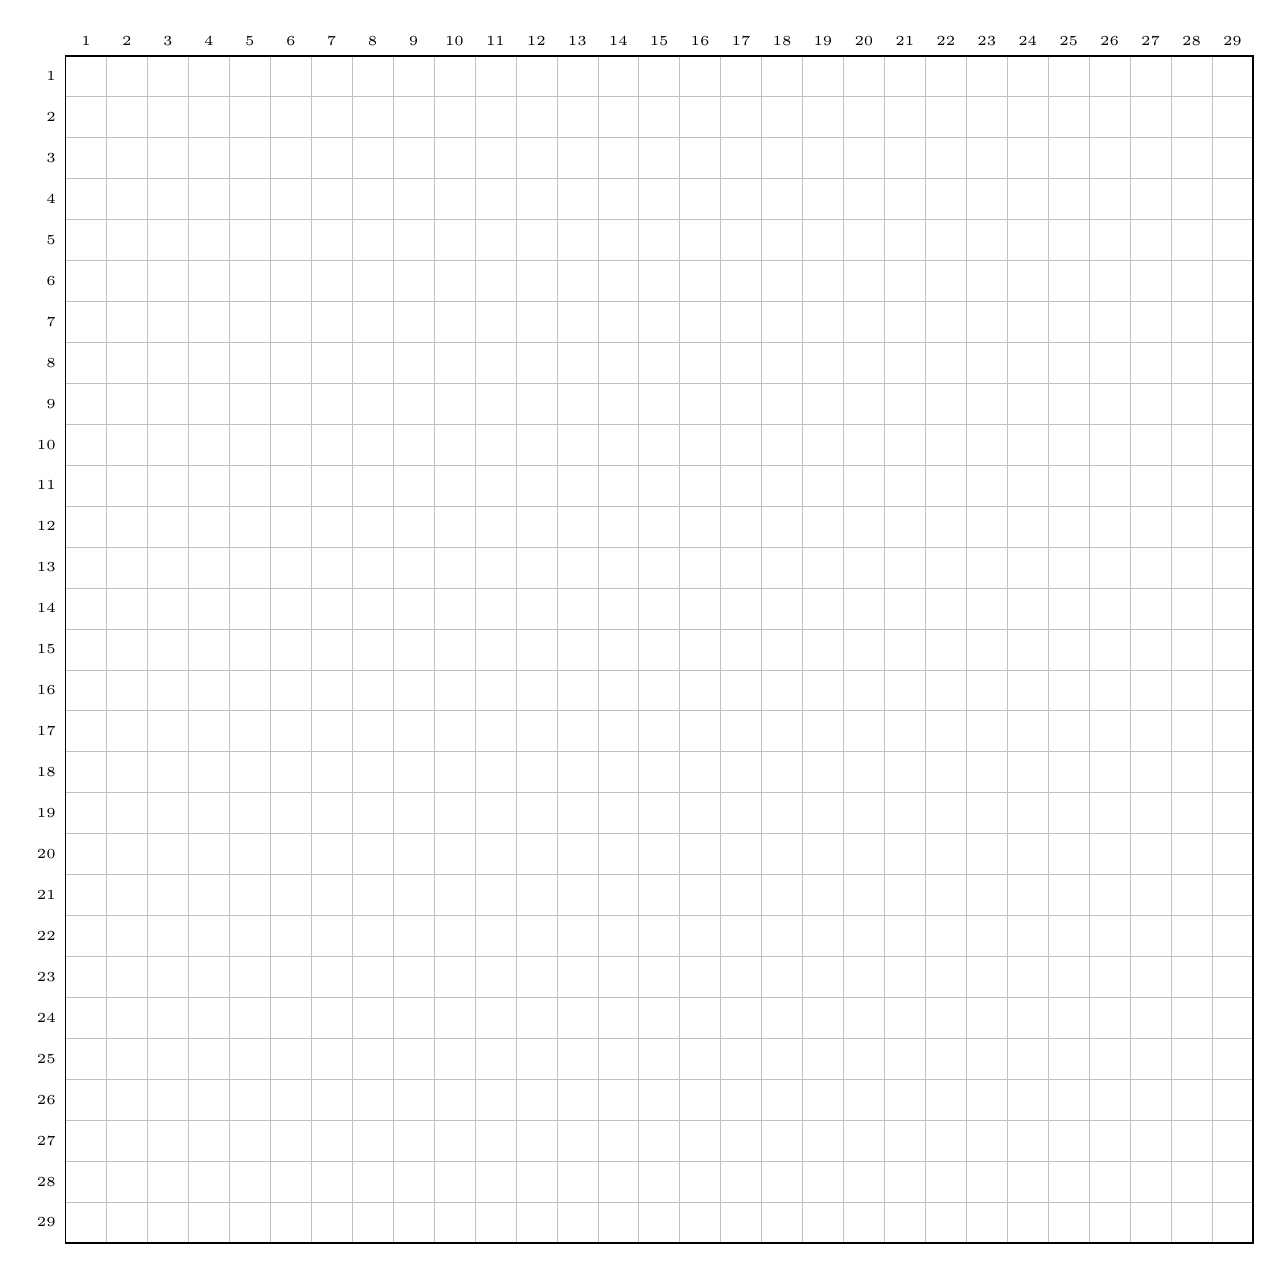
\begin{tikzpicture}[x=0.52cm,y=-0.52cm,font=\tiny]
\draw[gray!50,line width=0.2pt] (0,0) -- (0,29);
\draw[gray!50,line width=0.2pt] (1,0) -- (1,29);
\draw[gray!50,line width=0.2pt] (2,0) -- (2,29);
\draw[gray!50,line width=0.2pt] (3,0) -- (3,29);
\draw[gray!50,line width=0.2pt] (4,0) -- (4,29);
\draw[gray!50,line width=0.2pt] (5,0) -- (5,29);
\draw[gray!50,line width=0.2pt] (6,0) -- (6,29);
\draw[gray!50,line width=0.2pt] (7,0) -- (7,29);
\draw[gray!50,line width=0.2pt] (8,0) -- (8,29);
\draw[gray!50,line width=0.2pt] (9,0) -- (9,29);
\draw[gray!50,line width=0.2pt] (10,0) -- (10,29);
\draw[gray!50,line width=0.2pt] (11,0) -- (11,29);
\draw[gray!50,line width=0.2pt] (12,0) -- (12,29);
\draw[gray!50,line width=0.2pt] (13,0) -- (13,29);
\draw[gray!50,line width=0.2pt] (14,0) -- (14,29);
\draw[gray!50,line width=0.2pt] (15,0) -- (15,29);
\draw[gray!50,line width=0.2pt] (16,0) -- (16,29);
\draw[gray!50,line width=0.2pt] (17,0) -- (17,29);
\draw[gray!50,line width=0.2pt] (18,0) -- (18,29);
\draw[gray!50,line width=0.2pt] (19,0) -- (19,29);
\draw[gray!50,line width=0.2pt] (20,0) -- (20,29);
\draw[gray!50,line width=0.2pt] (21,0) -- (21,29);
\draw[gray!50,line width=0.2pt] (22,0) -- (22,29);
\draw[gray!50,line width=0.2pt] (23,0) -- (23,29);
\draw[gray!50,line width=0.2pt] (24,0) -- (24,29);
\draw[gray!50,line width=0.2pt] (25,0) -- (25,29);
\draw[gray!50,line width=0.2pt] (26,0) -- (26,29);
\draw[gray!50,line width=0.2pt] (27,0) -- (27,29);
\draw[gray!50,line width=0.2pt] (28,0) -- (28,29);
\draw[gray!50,line width=0.2pt] (29,0) -- (29,29);
\draw[gray!50,line width=0.2pt] (0,0) -- (29,0);
\draw[gray!50,line width=0.2pt] (0,1) -- (29,1);
\draw[gray!50,line width=0.2pt] (0,2) -- (29,2);
\draw[gray!50,line width=0.2pt] (0,3) -- (29,3);
\draw[gray!50,line width=0.2pt] (0,4) -- (29,4);
\draw[gray!50,line width=0.2pt] (0,5) -- (29,5);
\draw[gray!50,line width=0.2pt] (0,6) -- (29,6);
\draw[gray!50,line width=0.2pt] (0,7) -- (29,7);
\draw[gray!50,line width=0.2pt] (0,8) -- (29,8);
\draw[gray!50,line width=0.2pt] (0,9) -- (29,9);
\draw[gray!50,line width=0.2pt] (0,10) -- (29,10);
\draw[gray!50,line width=0.2pt] (0,11) -- (29,11);
\draw[gray!50,line width=0.2pt] (0,12) -- (29,12);
\draw[gray!50,line width=0.2pt] (0,13) -- (29,13);
\draw[gray!50,line width=0.2pt] (0,14) -- (29,14);
\draw[gray!50,line width=0.2pt] (0,15) -- (29,15);
\draw[gray!50,line width=0.2pt] (0,16) -- (29,16);
\draw[gray!50,line width=0.2pt] (0,17) -- (29,17);
\draw[gray!50,line width=0.2pt] (0,18) -- (29,18);
\draw[gray!50,line width=0.2pt] (0,19) -- (29,19);
\draw[gray!50,line width=0.2pt] (0,20) -- (29,20);
\draw[gray!50,line width=0.2pt] (0,21) -- (29,21);
\draw[gray!50,line width=0.2pt] (0,22) -- (29,22);
\draw[gray!50,line width=0.2pt] (0,23) -- (29,23);
\draw[gray!50,line width=0.2pt] (0,24) -- (29,24);
\draw[gray!50,line width=0.2pt] (0,25) -- (29,25);
\draw[gray!50,line width=0.2pt] (0,26) -- (29,26);
\draw[gray!50,line width=0.2pt] (0,27) -- (29,27);
\draw[gray!50,line width=0.2pt] (0,28) -- (29,28);
\draw[gray!50,line width=0.2pt] (0,29) -- (29,29);
\draw[black,line width=0.7pt] (0,0) rectangle (29,29);
\node[above] at (0.5,0) {\tiny 1};
\node[above] at (1.5,0) {\tiny 2};
\node[above] at (2.5,0) {\tiny 3};
\node[above] at (3.5,0) {\tiny 4};
\node[above] at (4.5,0) {\tiny 5};
\node[above] at (5.5,0) {\tiny 6};
\node[above] at (6.5,0) {\tiny 7};
\node[above] at (7.5,0) {\tiny 8};
\node[above] at (8.5,0) {\tiny 9};
\node[above] at (9.5,0) {\tiny 10};
\node[above] at (10.5,0) {\tiny 11};
\node[above] at (11.5,0) {\tiny 12};
\node[above] at (12.5,0) {\tiny 13};
\node[above] at (13.5,0) {\tiny 14};
\node[above] at (14.5,0) {\tiny 15};
\node[above] at (15.5,0) {\tiny 16};
\node[above] at (16.5,0) {\tiny 17};
\node[above] at (17.5,0) {\tiny 18};
\node[above] at (18.5,0) {\tiny 19};
\node[above] at (19.5,0) {\tiny 20};
\node[above] at (20.5,0) {\tiny 21};
\node[above] at (21.5,0) {\tiny 22};
\node[above] at (22.5,0) {\tiny 23};
\node[above] at (23.5,0) {\tiny 24};
\node[above] at (24.5,0) {\tiny 25};
\node[above] at (25.5,0) {\tiny 26};
\node[above] at (26.5,0) {\tiny 27};
\node[above] at (27.5,0) {\tiny 28};
\node[above] at (28.5,0) {\tiny 29};
\node[left] at (0,0.5) {\tiny 1};
\node[left] at (0,1.5) {\tiny 2};
\node[left] at (0,2.5) {\tiny 3};
\node[left] at (0,3.5) {\tiny 4};
\node[left] at (0,4.5) {\tiny 5};
\node[left] at (0,5.5) {\tiny 6};
\node[left] at (0,6.5) {\tiny 7};
\node[left] at (0,7.5) {\tiny 8};
\node[left] at (0,8.5) {\tiny 9};
\node[left] at (0,9.5) {\tiny 10};
\node[left] at (0,10.5) {\tiny 11};
\node[left] at (0,11.5) {\tiny 12};
\node[left] at (0,12.5) {\tiny 13};
\node[left] at (0,13.5) {\tiny 14};
\node[left] at (0,14.5) {\tiny 15};
\node[left] at (0,15.5) {\tiny 16};
\node[left] at (0,16.5) {\tiny 17};
\node[left] at (0,17.5) {\tiny 18};
\node[left] at (0,18.5) {\tiny 19};
\node[left] at (0,19.5) {\tiny 20};
\node[left] at (0,20.5) {\tiny 21};
\node[left] at (0,21.5) {\tiny 22};
\node[left] at (0,22.5) {\tiny 23};
\node[left] at (0,23.5) {\tiny 24};
\node[left] at (0,24.5) {\tiny 25};
\node[left] at (0,25.5) {\tiny 26};
\node[left] at (0,26.5) {\tiny 27};
\node[left] at (0,27.5) {\tiny 28};
\node[left] at (0,28.5) {\tiny 29};
\end{tikzpicture}
\end{center}

\newpage
\section{Fase 4 — Gauss-Jordan-eliminatie modulo 2}

Nu je zelf matrix $A$ hebt opgebouwd (Fase 2) en matrix $B$ hebt gedemaskeerd (Fase 3), is de rest identiek aan een klassiek stelsel: vind de unieke matrix $X$ (opnieuw $29\times 29$, enkel 0'en en 1'en) die voldoet aan
\[
A \cdot X \equiv B \pmod 2.
\]

Dit is de finale opgave: zodra je $X$ volledig hebt uitgeschreven, is de opdracht voltooid.

\begin{infobox}
\textbf{Waarom dit werkt.} Rekenen ``modulo 2'' betekent: elke optelling levert een 0 of een 1 op, nooit meer. Concreet is $1+1=0$, $1+0=1$, $0+0=0$ — dit is precies de logische \textsc{xor}-operatie. Matrices met enkel 0'en en 1'en, waarbij alle rekenwerk op deze manier gebeurt, leven in wat wiskundigen het \textbf{eindig veld $\mathrm{GF}(2)$} noemen (Galois-veld met 2 elementen). Alle vertrouwde regels van lineaire algebra — matrixvermenigvuldiging, Gauss-eliminatie, inverteerbaarheid — blijven gewoon geldig, alleen de optelling verandert. Deze wiskunde is de basis van cryptografie en codeertheorie in het algemeen.
\end{infobox}

\subsection{Het principe}
Om $X$ te vinden uit $AX \equiv B \pmod 2$, bouw je de \textbf{uitgebreide matrix} $[A \mid B]$ (matrix $A$ en matrix $B$ naast elkaar geplakt, samen dus $29 \times 58$). Door rijoperaties toe te passen — steeds modulo 2 — herleid je het linkerdeel $A$ tot de identiteitsmatrix $I$. Wat er dan rechts overblijft, is exact de gezochte matrix $X$:
\[
[A \mid B] \ \xrightarrow{\text{rijoperaties mod 2}}\ [I \mid X].
\]

\textbf{Toegelaten rijoperaties:}
\begin{enumerate}[label=(\roman*)]
\item Twee rijen verwisselen.
\item Eén rij optellen (\textsc{xor}) bij een andere rij.
\end{enumerate}
Vermenigvuldigen van een rij met een constante is hier overbodig: de enige niet-triviale constante modulo 2 is $1$ zelf, dus deze operatie doet niets.

\subsection{Het algoritme, stap voor stap}
\begin{enumerate}
\item Start bij kolom 1, rij 1.
\item Zoek in de huidige kolom (op of onder de huidige rij) een rij met een 1 in die kolom — dit wordt de \textbf{pivotrij}. Is er geen enkele 1 te vinden, ga naar de volgende kolom.
\item Verwissel indien nodig deze pivotrij met de huidige rij, zodat de pivot op de diagonaal staat.
\item Tel deze pivotrij (\textsc{xor}) op bij \emph{elke andere rij} die in deze kolom een 1 heeft — zowel erboven als eronder. Na deze stap staat er in de hele kolom nergens anders meer een 1 dan in de pivotrij zelf.
\item Ga naar de volgende rij en kolom, herhaal.
\item Na 29 succesvolle pivotstappen staat links $I$, en rechts staat $X$.
\end{enumerate}

\subsection{Volledig uitgewerkt minivoorbeeld (\texorpdfstring{$3\times 3$}{3x3})}
Om de methode te illustreren lossen we eerst een kleine versie op. Stel:
\[
A = \begin{pmatrix} 1&1&0\\0&1&1\\1&0&1\end{pmatrix}, \qquad
B = \begin{pmatrix} 1&0&1\\0&1&0\\1&1&1\end{pmatrix}.
\]
Uitgebreide matrix:
\[
[A\mid B] = \left(\begin{array}{ccc|ccc}
1&1&0&1&0&1\\
0&1&1&0&1&0\\
1&0&1&1&1&1
\end{array}\right)
\]

\textbf{Stap 1 — kolom 1.} Rij 1 heeft al een 1 op de diagonaal (pivot gevonden, geen verwisseling nodig). Tel rij 1 op bij elke andere rij die in kolom 1 een 1 heeft: dat is rij 3.
\[
R_3 \leftarrow R_3 + R_1 = (1{+}1,\,0{+}1,\,1{+}0 \mid 1{+}1,\,1{+}0,\,1{+}1) = (0,1,1\mid 0,1,0)
\]
Nieuwe matrix:
\[
\left(\begin{array}{ccc|ccc}
1&1&0&1&0&1\\
0&1&1&0&1&0\\
0&1&1&0&1&0
\end{array}\right)
\]

\textbf{Stap 2 — kolom 2.} Rij 2 heeft een 1 op de diagonaal. Tel rij 2 op bij elke andere rij met een 1 in kolom 2: dat zijn rij 1 én rij 3.
\[
R_1 \leftarrow R_1+R_2 = (1{+}0,1{+}1,0{+}1\mid 1{+}0,0{+}1,1{+}0) = (1,0,1\mid 1,1,1)
\]
\[
R_3 \leftarrow R_3+R_2 = (0{+}0,1{+}1,1{+}1\mid 0{+}0,1{+}1,0{+}0) = (0,0,0\mid 0,0,0)
\]
Nieuwe matrix:
\[
\left(\begin{array}{ccc|ccc}
1&0&1&1&1&1\\
0&1&1&0&1&0\\
0&0&0&0&0&0
\end{array}\right)
\]

Hier zien we dat rij 3 volledig nul is geworden in het linkerdeel — dit \emph{specifieke} kleine voorbeeld heeft dus een niet-inverteerbare $A$ (rang 2 in plaats van 3), en levert dus geen unieke oplossing. Dit minivoorbeeld illustreert enkel de rijoperaties zelf; in de echte puzzel hieronder is gegarandeerd dat $A$ volledig inverteerbaar is (rang 29), dus daar loop je dit probleem niet tegen het lijf — elke kolom krijgt gegarandeerd een pivot.

\begin{infobox}
\textbf{Controleer je werk onderweg.} Na elke pivotstap mag je gerust teruggaan en met de hand $A\cdot X \stackrel{?}{\equiv} B$ verifiëren op een paar losse rijen — dat is veel sneller dan de hele eliminatie opnieuw te doen, en vangt rekenfouten vroeg op.
\end{infobox}

\begin{landscape}
\newpage
\subsection{Werkblad — de uitgebreide matrix \texorpdfstring{$[A\mid B]$}{[A|B]} (29 × 58)}
Dit is je volledige werkruimte: matrix $A$ (links) en matrix $B$ (rechts) naast elkaar, precies zoals in \S5.1 beschreven. Voer hier je rijoperaties uit totdat het linkerdeel de identiteitsmatrix $I$ is geworden — wat dan rechts overblijft, is $X$.

\begin{center}
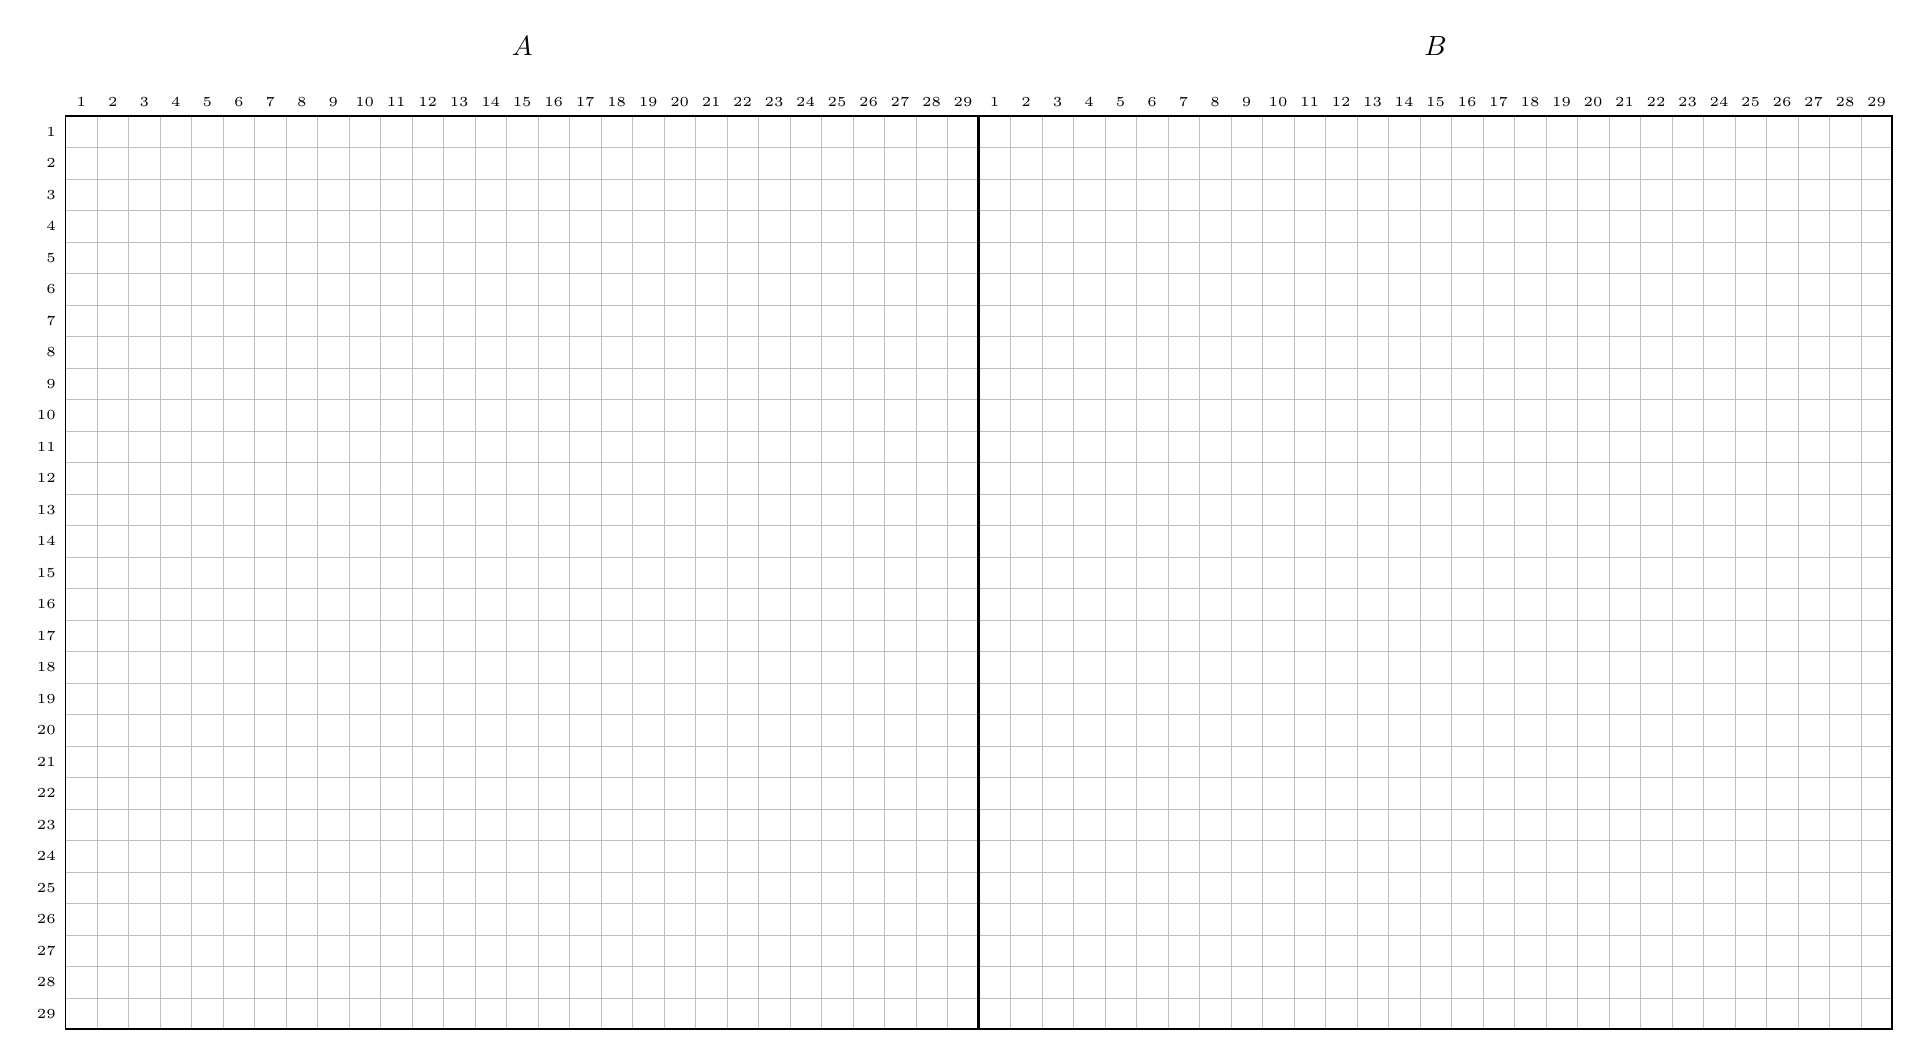
\begin{tikzpicture}[x=0.4cm,y=-0.4cm,font=\tiny]
\draw[gray!50,line width=0.2pt] (0,0) -- (0,29);
\draw[gray!50,line width=0.2pt] (1,0) -- (1,29);
\draw[gray!50,line width=0.2pt] (2,0) -- (2,29);
\draw[gray!50,line width=0.2pt] (3,0) -- (3,29);
\draw[gray!50,line width=0.2pt] (4,0) -- (4,29);
\draw[gray!50,line width=0.2pt] (5,0) -- (5,29);
\draw[gray!50,line width=0.2pt] (6,0) -- (6,29);
\draw[gray!50,line width=0.2pt] (7,0) -- (7,29);
\draw[gray!50,line width=0.2pt] (8,0) -- (8,29);
\draw[gray!50,line width=0.2pt] (9,0) -- (9,29);
\draw[gray!50,line width=0.2pt] (10,0) -- (10,29);
\draw[gray!50,line width=0.2pt] (11,0) -- (11,29);
\draw[gray!50,line width=0.2pt] (12,0) -- (12,29);
\draw[gray!50,line width=0.2pt] (13,0) -- (13,29);
\draw[gray!50,line width=0.2pt] (14,0) -- (14,29);
\draw[gray!50,line width=0.2pt] (15,0) -- (15,29);
\draw[gray!50,line width=0.2pt] (16,0) -- (16,29);
\draw[gray!50,line width=0.2pt] (17,0) -- (17,29);
\draw[gray!50,line width=0.2pt] (18,0) -- (18,29);
\draw[gray!50,line width=0.2pt] (19,0) -- (19,29);
\draw[gray!50,line width=0.2pt] (20,0) -- (20,29);
\draw[gray!50,line width=0.2pt] (21,0) -- (21,29);
\draw[gray!50,line width=0.2pt] (22,0) -- (22,29);
\draw[gray!50,line width=0.2pt] (23,0) -- (23,29);
\draw[gray!50,line width=0.2pt] (24,0) -- (24,29);
\draw[gray!50,line width=0.2pt] (25,0) -- (25,29);
\draw[gray!50,line width=0.2pt] (26,0) -- (26,29);
\draw[gray!50,line width=0.2pt] (27,0) -- (27,29);
\draw[gray!50,line width=0.2pt] (28,0) -- (28,29);
\draw[gray!50,line width=0.2pt] (29,0) -- (29,29);
\draw[gray!50,line width=0.2pt] (30,0) -- (30,29);
\draw[gray!50,line width=0.2pt] (31,0) -- (31,29);
\draw[gray!50,line width=0.2pt] (32,0) -- (32,29);
\draw[gray!50,line width=0.2pt] (33,0) -- (33,29);
\draw[gray!50,line width=0.2pt] (34,0) -- (34,29);
\draw[gray!50,line width=0.2pt] (35,0) -- (35,29);
\draw[gray!50,line width=0.2pt] (36,0) -- (36,29);
\draw[gray!50,line width=0.2pt] (37,0) -- (37,29);
\draw[gray!50,line width=0.2pt] (38,0) -- (38,29);
\draw[gray!50,line width=0.2pt] (39,0) -- (39,29);
\draw[gray!50,line width=0.2pt] (40,0) -- (40,29);
\draw[gray!50,line width=0.2pt] (41,0) -- (41,29);
\draw[gray!50,line width=0.2pt] (42,0) -- (42,29);
\draw[gray!50,line width=0.2pt] (43,0) -- (43,29);
\draw[gray!50,line width=0.2pt] (44,0) -- (44,29);
\draw[gray!50,line width=0.2pt] (45,0) -- (45,29);
\draw[gray!50,line width=0.2pt] (46,0) -- (46,29);
\draw[gray!50,line width=0.2pt] (47,0) -- (47,29);
\draw[gray!50,line width=0.2pt] (48,0) -- (48,29);
\draw[gray!50,line width=0.2pt] (49,0) -- (49,29);
\draw[gray!50,line width=0.2pt] (50,0) -- (50,29);
\draw[gray!50,line width=0.2pt] (51,0) -- (51,29);
\draw[gray!50,line width=0.2pt] (52,0) -- (52,29);
\draw[gray!50,line width=0.2pt] (53,0) -- (53,29);
\draw[gray!50,line width=0.2pt] (54,0) -- (54,29);
\draw[gray!50,line width=0.2pt] (55,0) -- (55,29);
\draw[gray!50,line width=0.2pt] (56,0) -- (56,29);
\draw[gray!50,line width=0.2pt] (57,0) -- (57,29);
\draw[gray!50,line width=0.2pt] (58,0) -- (58,29);
\draw[gray!50,line width=0.2pt] (0,0) -- (58,0);
\draw[gray!50,line width=0.2pt] (0,1) -- (58,1);
\draw[gray!50,line width=0.2pt] (0,2) -- (58,2);
\draw[gray!50,line width=0.2pt] (0,3) -- (58,3);
\draw[gray!50,line width=0.2pt] (0,4) -- (58,4);
\draw[gray!50,line width=0.2pt] (0,5) -- (58,5);
\draw[gray!50,line width=0.2pt] (0,6) -- (58,6);
\draw[gray!50,line width=0.2pt] (0,7) -- (58,7);
\draw[gray!50,line width=0.2pt] (0,8) -- (58,8);
\draw[gray!50,line width=0.2pt] (0,9) -- (58,9);
\draw[gray!50,line width=0.2pt] (0,10) -- (58,10);
\draw[gray!50,line width=0.2pt] (0,11) -- (58,11);
\draw[gray!50,line width=0.2pt] (0,12) -- (58,12);
\draw[gray!50,line width=0.2pt] (0,13) -- (58,13);
\draw[gray!50,line width=0.2pt] (0,14) -- (58,14);
\draw[gray!50,line width=0.2pt] (0,15) -- (58,15);
\draw[gray!50,line width=0.2pt] (0,16) -- (58,16);
\draw[gray!50,line width=0.2pt] (0,17) -- (58,17);
\draw[gray!50,line width=0.2pt] (0,18) -- (58,18);
\draw[gray!50,line width=0.2pt] (0,19) -- (58,19);
\draw[gray!50,line width=0.2pt] (0,20) -- (58,20);
\draw[gray!50,line width=0.2pt] (0,21) -- (58,21);
\draw[gray!50,line width=0.2pt] (0,22) -- (58,22);
\draw[gray!50,line width=0.2pt] (0,23) -- (58,23);
\draw[gray!50,line width=0.2pt] (0,24) -- (58,24);
\draw[gray!50,line width=0.2pt] (0,25) -- (58,25);
\draw[gray!50,line width=0.2pt] (0,26) -- (58,26);
\draw[gray!50,line width=0.2pt] (0,27) -- (58,27);
\draw[gray!50,line width=0.2pt] (0,28) -- (58,28);
\draw[gray!50,line width=0.2pt] (0,29) -- (58,29);
\draw[black,line width=0.7pt] (0,0) rectangle (58,29);
\draw[black,line width=1.1pt] (29,0) -- (29,29);
\node[above] at (0.5,0) {\tiny 1};
\node[above] at (1.5,0) {\tiny 2};
\node[above] at (2.5,0) {\tiny 3};
\node[above] at (3.5,0) {\tiny 4};
\node[above] at (4.5,0) {\tiny 5};
\node[above] at (5.5,0) {\tiny 6};
\node[above] at (6.5,0) {\tiny 7};
\node[above] at (7.5,0) {\tiny 8};
\node[above] at (8.5,0) {\tiny 9};
\node[above] at (9.5,0) {\tiny 10};
\node[above] at (10.5,0) {\tiny 11};
\node[above] at (11.5,0) {\tiny 12};
\node[above] at (12.5,0) {\tiny 13};
\node[above] at (13.5,0) {\tiny 14};
\node[above] at (14.5,0) {\tiny 15};
\node[above] at (15.5,0) {\tiny 16};
\node[above] at (16.5,0) {\tiny 17};
\node[above] at (17.5,0) {\tiny 18};
\node[above] at (18.5,0) {\tiny 19};
\node[above] at (19.5,0) {\tiny 20};
\node[above] at (20.5,0) {\tiny 21};
\node[above] at (21.5,0) {\tiny 22};
\node[above] at (22.5,0) {\tiny 23};
\node[above] at (23.5,0) {\tiny 24};
\node[above] at (24.5,0) {\tiny 25};
\node[above] at (25.5,0) {\tiny 26};
\node[above] at (26.5,0) {\tiny 27};
\node[above] at (27.5,0) {\tiny 28};
\node[above] at (28.5,0) {\tiny 29};
\node[above] at (29.5,0) {\tiny 1};
\node[above] at (30.5,0) {\tiny 2};
\node[above] at (31.5,0) {\tiny 3};
\node[above] at (32.5,0) {\tiny 4};
\node[above] at (33.5,0) {\tiny 5};
\node[above] at (34.5,0) {\tiny 6};
\node[above] at (35.5,0) {\tiny 7};
\node[above] at (36.5,0) {\tiny 8};
\node[above] at (37.5,0) {\tiny 9};
\node[above] at (38.5,0) {\tiny 10};
\node[above] at (39.5,0) {\tiny 11};
\node[above] at (40.5,0) {\tiny 12};
\node[above] at (41.5,0) {\tiny 13};
\node[above] at (42.5,0) {\tiny 14};
\node[above] at (43.5,0) {\tiny 15};
\node[above] at (44.5,0) {\tiny 16};
\node[above] at (45.5,0) {\tiny 17};
\node[above] at (46.5,0) {\tiny 18};
\node[above] at (47.5,0) {\tiny 19};
\node[above] at (48.5,0) {\tiny 20};
\node[above] at (49.5,0) {\tiny 21};
\node[above] at (50.5,0) {\tiny 22};
\node[above] at (51.5,0) {\tiny 23};
\node[above] at (52.5,0) {\tiny 24};
\node[above] at (53.5,0) {\tiny 25};
\node[above] at (54.5,0) {\tiny 26};
\node[above] at (55.5,0) {\tiny 27};
\node[above] at (56.5,0) {\tiny 28};
\node[above] at (57.5,0) {\tiny 29};
\node[left] at (0,0.5) {\tiny 1};
\node[left] at (0,1.5) {\tiny 2};
\node[left] at (0,2.5) {\tiny 3};
\node[left] at (0,3.5) {\tiny 4};
\node[left] at (0,4.5) {\tiny 5};
\node[left] at (0,5.5) {\tiny 6};
\node[left] at (0,6.5) {\tiny 7};
\node[left] at (0,7.5) {\tiny 8};
\node[left] at (0,8.5) {\tiny 9};
\node[left] at (0,9.5) {\tiny 10};
\node[left] at (0,10.5) {\tiny 11};
\node[left] at (0,11.5) {\tiny 12};
\node[left] at (0,12.5) {\tiny 13};
\node[left] at (0,13.5) {\tiny 14};
\node[left] at (0,14.5) {\tiny 15};
\node[left] at (0,15.5) {\tiny 16};
\node[left] at (0,16.5) {\tiny 17};
\node[left] at (0,17.5) {\tiny 18};
\node[left] at (0,18.5) {\tiny 19};
\node[left] at (0,19.5) {\tiny 20};
\node[left] at (0,20.5) {\tiny 21};
\node[left] at (0,21.5) {\tiny 22};
\node[left] at (0,22.5) {\tiny 23};
\node[left] at (0,23.5) {\tiny 24};
\node[left] at (0,24.5) {\tiny 25};
\node[left] at (0,25.5) {\tiny 26};
\node[left] at (0,26.5) {\tiny 27};
\node[left] at (0,27.5) {\tiny 28};
\node[left] at (0,28.5) {\tiny 29};
\node[above,font=\normalsize\bfseries] at (14.5,-1.6) {$A$};
\node[above,font=\normalsize\bfseries] at (43.5,-1.6) {$B$};
\end{tikzpicture}
\end{center}

\vspace{0.3cm}
\textit{Tip: bij 29 pivotstappen op een matrix van deze breedte is één werkblad meestal niet genoeg — gebruik gerust los papier om de matrix na elke stap of elke paar stappen opnieuw over te schrijven, en bewaar dit blad als startpositie.}
\end{landscape}

\newpage
\subsection{Invulrooster — eindresultaat \texorpdfstring{$X$}{X}}
Noteer hier, na de volledige Gauss-Jordan-eliminatie op de echte $29\times 29$-matrices $A$ en $B$, de rechterhelft van de gereduceerde uitgebreide matrix — dit is je volledige eindresultaat $X$.

\begin{center}
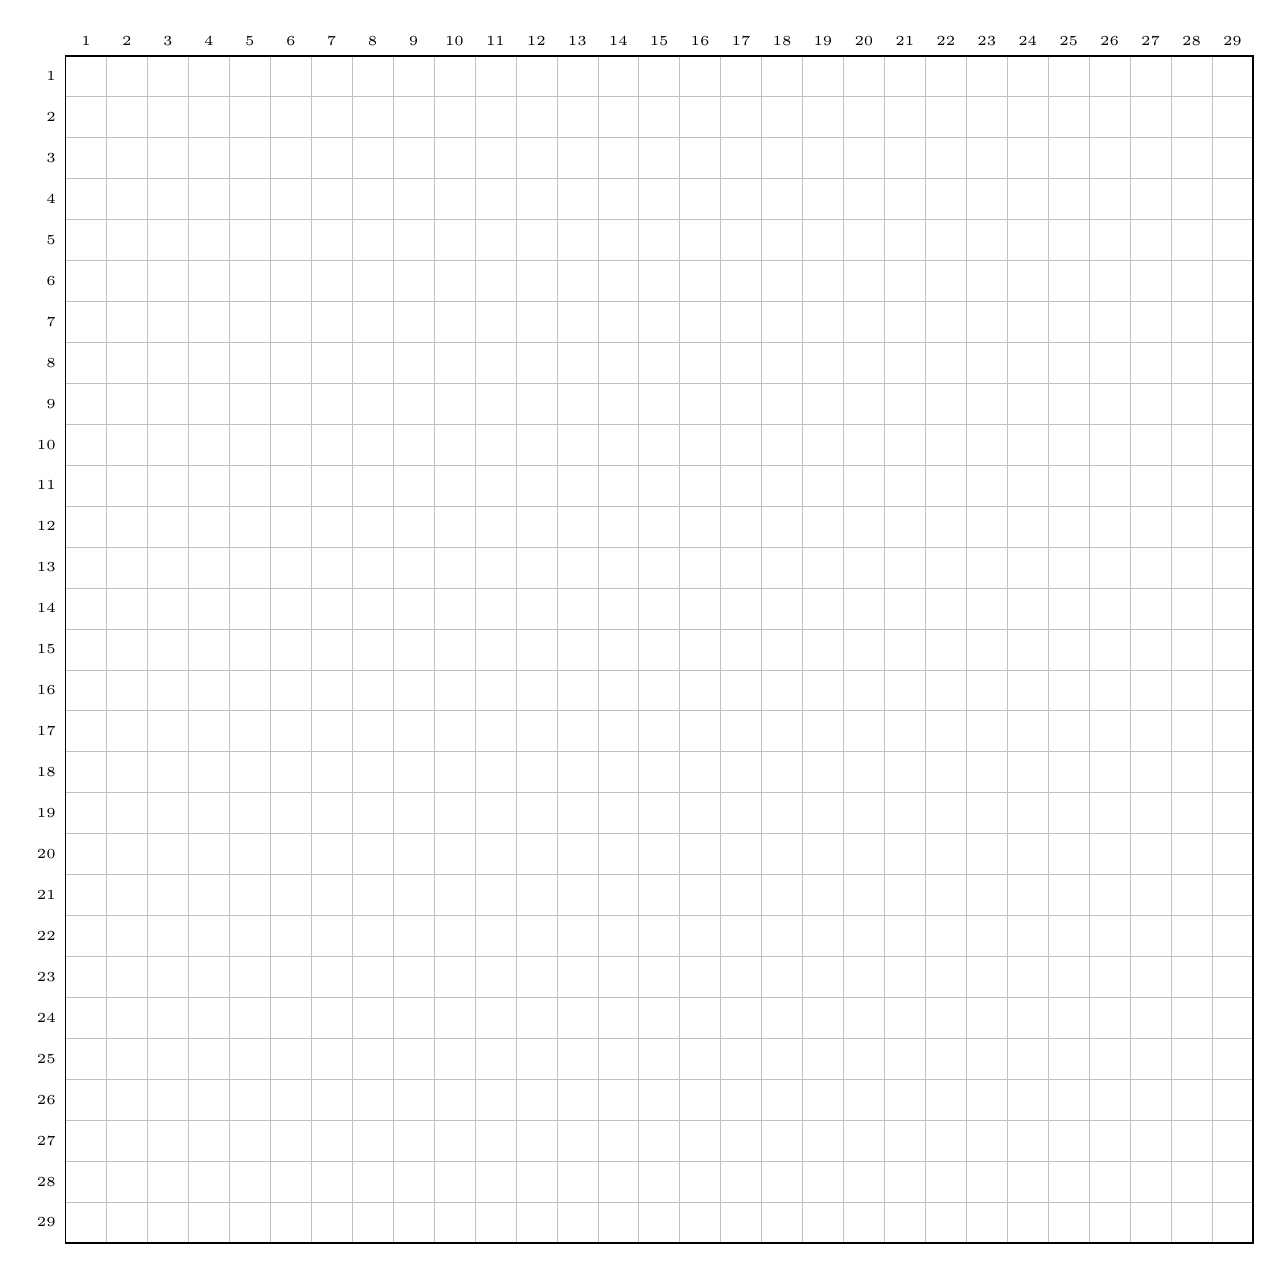
\begin{tikzpicture}[x=0.52cm,y=-0.52cm,font=\tiny]
\draw[gray!50,line width=0.2pt] (0,0) -- (0,29);
\draw[gray!50,line width=0.2pt] (1,0) -- (1,29);
\draw[gray!50,line width=0.2pt] (2,0) -- (2,29);
\draw[gray!50,line width=0.2pt] (3,0) -- (3,29);
\draw[gray!50,line width=0.2pt] (4,0) -- (4,29);
\draw[gray!50,line width=0.2pt] (5,0) -- (5,29);
\draw[gray!50,line width=0.2pt] (6,0) -- (6,29);
\draw[gray!50,line width=0.2pt] (7,0) -- (7,29);
\draw[gray!50,line width=0.2pt] (8,0) -- (8,29);
\draw[gray!50,line width=0.2pt] (9,0) -- (9,29);
\draw[gray!50,line width=0.2pt] (10,0) -- (10,29);
\draw[gray!50,line width=0.2pt] (11,0) -- (11,29);
\draw[gray!50,line width=0.2pt] (12,0) -- (12,29);
\draw[gray!50,line width=0.2pt] (13,0) -- (13,29);
\draw[gray!50,line width=0.2pt] (14,0) -- (14,29);
\draw[gray!50,line width=0.2pt] (15,0) -- (15,29);
\draw[gray!50,line width=0.2pt] (16,0) -- (16,29);
\draw[gray!50,line width=0.2pt] (17,0) -- (17,29);
\draw[gray!50,line width=0.2pt] (18,0) -- (18,29);
\draw[gray!50,line width=0.2pt] (19,0) -- (19,29);
\draw[gray!50,line width=0.2pt] (20,0) -- (20,29);
\draw[gray!50,line width=0.2pt] (21,0) -- (21,29);
\draw[gray!50,line width=0.2pt] (22,0) -- (22,29);
\draw[gray!50,line width=0.2pt] (23,0) -- (23,29);
\draw[gray!50,line width=0.2pt] (24,0) -- (24,29);
\draw[gray!50,line width=0.2pt] (25,0) -- (25,29);
\draw[gray!50,line width=0.2pt] (26,0) -- (26,29);
\draw[gray!50,line width=0.2pt] (27,0) -- (27,29);
\draw[gray!50,line width=0.2pt] (28,0) -- (28,29);
\draw[gray!50,line width=0.2pt] (29,0) -- (29,29);
\draw[gray!50,line width=0.2pt] (0,0) -- (29,0);
\draw[gray!50,line width=0.2pt] (0,1) -- (29,1);
\draw[gray!50,line width=0.2pt] (0,2) -- (29,2);
\draw[gray!50,line width=0.2pt] (0,3) -- (29,3);
\draw[gray!50,line width=0.2pt] (0,4) -- (29,4);
\draw[gray!50,line width=0.2pt] (0,5) -- (29,5);
\draw[gray!50,line width=0.2pt] (0,6) -- (29,6);
\draw[gray!50,line width=0.2pt] (0,7) -- (29,7);
\draw[gray!50,line width=0.2pt] (0,8) -- (29,8);
\draw[gray!50,line width=0.2pt] (0,9) -- (29,9);
\draw[gray!50,line width=0.2pt] (0,10) -- (29,10);
\draw[gray!50,line width=0.2pt] (0,11) -- (29,11);
\draw[gray!50,line width=0.2pt] (0,12) -- (29,12);
\draw[gray!50,line width=0.2pt] (0,13) -- (29,13);
\draw[gray!50,line width=0.2pt] (0,14) -- (29,14);
\draw[gray!50,line width=0.2pt] (0,15) -- (29,15);
\draw[gray!50,line width=0.2pt] (0,16) -- (29,16);
\draw[gray!50,line width=0.2pt] (0,17) -- (29,17);
\draw[gray!50,line width=0.2pt] (0,18) -- (29,18);
\draw[gray!50,line width=0.2pt] (0,19) -- (29,19);
\draw[gray!50,line width=0.2pt] (0,20) -- (29,20);
\draw[gray!50,line width=0.2pt] (0,21) -- (29,21);
\draw[gray!50,line width=0.2pt] (0,22) -- (29,22);
\draw[gray!50,line width=0.2pt] (0,23) -- (29,23);
\draw[gray!50,line width=0.2pt] (0,24) -- (29,24);
\draw[gray!50,line width=0.2pt] (0,25) -- (29,25);
\draw[gray!50,line width=0.2pt] (0,26) -- (29,26);
\draw[gray!50,line width=0.2pt] (0,27) -- (29,27);
\draw[gray!50,line width=0.2pt] (0,28) -- (29,28);
\draw[gray!50,line width=0.2pt] (0,29) -- (29,29);
\draw[black,line width=0.7pt] (0,0) rectangle (29,29);
\node[above] at (0.5,0) {\tiny 1};
\node[above] at (1.5,0) {\tiny 2};
\node[above] at (2.5,0) {\tiny 3};
\node[above] at (3.5,0) {\tiny 4};
\node[above] at (4.5,0) {\tiny 5};
\node[above] at (5.5,0) {\tiny 6};
\node[above] at (6.5,0) {\tiny 7};
\node[above] at (7.5,0) {\tiny 8};
\node[above] at (8.5,0) {\tiny 9};
\node[above] at (9.5,0) {\tiny 10};
\node[above] at (10.5,0) {\tiny 11};
\node[above] at (11.5,0) {\tiny 12};
\node[above] at (12.5,0) {\tiny 13};
\node[above] at (13.5,0) {\tiny 14};
\node[above] at (14.5,0) {\tiny 15};
\node[above] at (15.5,0) {\tiny 16};
\node[above] at (16.5,0) {\tiny 17};
\node[above] at (17.5,0) {\tiny 18};
\node[above] at (18.5,0) {\tiny 19};
\node[above] at (19.5,0) {\tiny 20};
\node[above] at (20.5,0) {\tiny 21};
\node[above] at (21.5,0) {\tiny 22};
\node[above] at (22.5,0) {\tiny 23};
\node[above] at (23.5,0) {\tiny 24};
\node[above] at (24.5,0) {\tiny 25};
\node[above] at (25.5,0) {\tiny 26};
\node[above] at (26.5,0) {\tiny 27};
\node[above] at (27.5,0) {\tiny 28};
\node[above] at (28.5,0) {\tiny 29};
\node[left] at (0,0.5) {\tiny 1};
\node[left] at (0,1.5) {\tiny 2};
\node[left] at (0,2.5) {\tiny 3};
\node[left] at (0,3.5) {\tiny 4};
\node[left] at (0,4.5) {\tiny 5};
\node[left] at (0,5.5) {\tiny 6};
\node[left] at (0,6.5) {\tiny 7};
\node[left] at (0,7.5) {\tiny 8};
\node[left] at (0,8.5) {\tiny 9};
\node[left] at (0,9.5) {\tiny 10};
\node[left] at (0,10.5) {\tiny 11};
\node[left] at (0,11.5) {\tiny 12};
\node[left] at (0,12.5) {\tiny 13};
\node[left] at (0,13.5) {\tiny 14};
\node[left] at (0,14.5) {\tiny 15};
\node[left] at (0,15.5) {\tiny 16};
\node[left] at (0,16.5) {\tiny 17};
\node[left] at (0,17.5) {\tiny 18};
\node[left] at (0,18.5) {\tiny 19};
\node[left] at (0,19.5) {\tiny 20};
\node[left] at (0,20.5) {\tiny 21};
\node[left] at (0,21.5) {\tiny 22};
\node[left] at (0,22.5) {\tiny 23};
\node[left] at (0,23.5) {\tiny 24};
\node[left] at (0,24.5) {\tiny 25};
\node[left] at (0,25.5) {\tiny 26};
\node[left] at (0,26.5) {\tiny 27};
\node[left] at (0,27.5) {\tiny 28};
\node[left] at (0,28.5) {\tiny 29};
\end{tikzpicture}
\end{center}

\end{document}
